% I seguenti commenti speciali impostano:
% 1. 
% 2. PDFLaTeX come motore di composizione;
% 3. tesi.tex come documento principale;
% 4. il controllo ortografico italiano per l'editor.

% !TEX encoding = UTF-8
% !TEX TS-program = pdflatex
% !TEX root = tesi.tex
% !TEX spellcheck = it-IT
%!TEX program = xelatex
\documentclass[11pt,                    % corpo del font principale
    a4paper,                 % carta A4
    twoside,                 % impagina per fronte-retro
    openright,               % inizio capitoli a destra
    english,
    ctexart,
]{book}

%**************************************************************
% Importazione package
%************************************************************** 
%\usepackage{amsmath,amssymb,amsthm}    % matematica
\usepackage[UTF8]{ctex}
\usepackage[T1]{fontenc}                % codifica dei font:
% NOTA BENE! richiede una distribuzione *completa* di LaTeX

\usepackage[utf8]{inputenc}             % codifica di input; anche [latin1] va bene
% NOTA BENE! va accordata con le preferenze dell'editor

\usepackage[english]{babel}    % per scrivere in italiano e in inglese;
% l'ultima lingua (l'italiano) risulta predefinita

\usepackage{bookmark}                   % segnalibri

\usepackage{caption}                    % didascalie

\usepackage{chngpage,calc}              % centra il frontespizio

\usepackage{csquotes}                   % gestisce automaticamente i caratteri (")

\usepackage{emptypage}                  % pagine vuote senza testatina e piede di pagina

\usepackage{epigraph}            % per epigrafi

\usepackage{eurosym}                    % simbolo dell'euro

%\usepackage{indentfirst}               % rientra il primo paragrafo di ogni sezione

\usepackage{graphicx}                   % immagini

\usepackage{hyperref}                   % collegamenti ipertestuali

\usepackage[binding=5mm]{layaureo}      % margini ottimizzati per l'A4; rilegatura di 5 mm


\usepackage{microtype}                  % microtipografia

\usepackage{mparhack,fixltx2e,relsize}  % finezze tipografiche

\usepackage{nameref}                    % visualizza nome dei riferimenti                                      

\usepackage[font=small]{quoting}        % citazioni

%\usepackage{subfig}                     % sottofigure, sottotabelle

\usepackage[english]{varioref}          % riferimenti completi della pagina

\usepackage[dvipsnames]{xcolor}         % colori
\usepackage{formattazione}

\usepackage{booktabs}                   % tabelle                                       
\usepackage{tabularx}                   % tabelle di larghezza prefissata                                    
\usepackage{longtable}                  % tabelle su più pagine                                        
\usepackage{ltxtable}                   % tabelle su più pagine e adattabili in larghezza

\usepackage{multicol}                   % colonne multiple
\usepackage{tabularx}

\usepackage[toc, acronym]{glossaries}   % glossario
% per includerlo nel documento bisogna:
% 1. compilare una prima volta tesi.tex;
% 2. eseguire: makeindex -s tesi.ist -t tesi.glg -o tesi.gls tesi.glo
% 3. eseguire: makeindex -s tesi.ist -t tesi.alg -o tesi.acr tesi.acn
% 4. compilare due volte tesi.tex.
\usepackage[backend=biber,style=numeric-comp,hyperref,backref]{biblatex}
% eccellente pacchetto per la bibliografia;
% produce uno stile di citazione autore-anno;
% lo stile "numeric-comp" produce riferimenti numerici
% per includerlo nel documento bisogna:
% 1. compilare una prima volta tesi.tex;
% 2. eseguire: biber tesi
% 3. compilare ancora tesi.tex.

%**************************************************************
% file contenente le impostazioni della tesi
%**************************************************************

%**************************************************************
% Frontespizio
%**************************************************************

% Autore
\newcommand{\myName}{Giuseppe Murro}
\newcommand{\myTitle}{SynBA: A contextualized Synonym-Based adversarial Attack \\for Text Classification}

% Tipo di tesi                   
\newcommand{\myDegree}{Final Thesis}

% Università             
\newcommand{\myUni}{Alma Mater Studiorum - University of Bologna}

% Facoltà       
\newcommand{\myFaculty}{Master's Degree in Artificial Intelligence}

% Dipartimento
\newcommand{\myDepartment}{Department of Computer Science and Engineering}

% Titolo del relatore
\newcommand{\profTitle}{Prof. }

% Relatore
\newcommand{\myProf}{Paolo Torroni}

% Luogo
\newcommand{\myLocation}{Bologna}

% Anno accademico
\newcommand{\myAA}{2021-2022}

% Data discussione
\newcommand{\myTime}{06 December 2022}


\addto\captionsenglish{\renewcommand{\lstlistingname}{Code}}

%**************************************************************
% Impostazioni di impaginazione
% see: http://wwwcdf.pd.infn.it/AppuntiLinux/a2547.htm
%**************************************************************

\setlength{\parindent}{14pt}   % larghezza rientro della prima riga
\setlength{\parskip}{0pt}   % distanza tra i paragrafi


%**************************************************************
% Impostazioni di biblatex
%**************************************************************
\bibliography{bibliografia} % database di biblatex 

\defbibheading{bibliography} {
    \cleardoublepage
    \phantomsection 
    %\addcontentsline{toc}{chapter}{\bibname}
    \chapter*{\bibname\markboth{\bibname}{\bibname}}
}

\setlength\bibitemsep{1.5\itemsep} % spazio tra entry

\DeclareBibliographyCategory{opere}
\DeclareBibliographyCategory{web}

\addtocategory{opere}{womak:lean-thinking}
\addtocategory{web}{site:agile-manifesto}

\defbibheading{opere}{\section*{Bibliography}}
\defbibheading{web}{\section*{Websites}}


%**************************************************************
% Impostazioni di caption
%**************************************************************
\captionsetup{
    tableposition=top,
    figureposition=bottom,
    font=small,
    format=hang,
    labelfont=bf
}

%**************************************************************
% Impostazioni di glossaries
%**************************************************************
\input{Glossario} % database di termini
\makeglossaries


%**************************************************************
% Impostazioni di graphicx
%**************************************************************
\graphicspath{{images/}} % cartella dove sono riposte le immagini


%**************************************************************
% Impostazioni di hyperref
%**************************************************************
\hypersetup{
    %hyperfootnotes=false,
    %pdfpagelabels,
    %draft,	% = elimina tutti i link (utile per stampe in bianco e nero)
    colorlinks=true,
    linktocpage=true,
    pdfstartpage=1,
    pdfstartview=FitV,
    % decommenta la riga seguente per avere link in nero (per esempio per la stampa in bianco e nero)
    %colorlinks=false, linktocpage=false, pdfborder={0 0 0}, pdfstartpage=1, pdfstartview=FitV,
    breaklinks=true,
    pdfpagemode=UseNone,
    pageanchor=true,
    pdfpagemode=UseOutlines,
    plainpages=false,
    bookmarksnumbered,
    bookmarksopen=true,
    bookmarksopenlevel=1,
    hypertexnames=true,
    pdfhighlight=/O,
    %nesting=true,
    %frenchlinks,
    urlcolor=webbrown,
    linkcolor=RoyalBlue,
    citecolor=webgreen,
    %pagecolor=RoyalBlue,
    %urlcolor=Black, linkcolor=Black, citecolor=Black, %pagecolor=Black,
    pdftitle={\myTitle},
    pdfauthor={\textcopyright\ \myName, \myUni, \myFaculty},
    pdfsubject={},
    pdfkeywords={},
    pdfcreator={pdfLaTeX},
    pdfproducer={LaTeX}
}

%**************************************************************
% Impostazioni di listings
%**************************************************************
\lstset{
    language=[LaTeX]Tex,%C++,
    keywordstyle=\color{RoyalBlue}, %\bfseries,
    basicstyle=\small\ttfamily,
    %identifierstyle=\color{NavyBlue},
    commentstyle=\color{Green}\ttfamily,
    stringstyle=\rmfamily,
    numbers=none, %left,%
    numberstyle=\scriptsize, %\tiny
    stepnumber=5,
    numbersep=8pt,
    showstringspaces=false,
    breaklines=true,
    frameround=ftff,
    frame=single
} 


%**************************************************************
% Impostazioni di xcolor
%**************************************************************
\definecolor{webgreen}{rgb}{0,.5,0}
\definecolor{webbrown}{rgb}{.6,0,0}
\usepackage{chngcntr}
\counterwithout{footnote}{chapter}

%**************************************************************
% Altro
%**************************************************************

\newcommand{\omissis}{[\dots\negthinspace]} % produce [...]

% eccezioni all'algoritmo di sillabazione
\hyphenation
{
    ma-cro-istru-zio-ne
    gi-ral-din
}

\newcommand{\sectionname}{Section}
\addto\captions{\renewcommand{\figurename}{Figure}
                       \renewcommand{\tablename}{Table}}

\newcommand{\glsfirstoccur}{\ap{{[g]}}}

\newcommand{\intro}[1]{\emph{\textsf{#1}}}

%**************************************************************
% Environment per ``namespace description''
%**************************************************************

\newenvironment{namespacedesc}{
    \vspace{10pt}
    \par \noindent                              % start new paragraph
    \begin{description} 
}{
    \end{description}
    \medskip
}

\newcommand{\classdesc}[2]{\item[\textbf{#1:}] #2}
\renewcommand{\labelitemi}{$\bullet$}
\renewcommand{\labelitemii}{$\circ$}
\renewcommand{\labelitemiii}{-}
\renewcommand{\labelitemiv}{$\cdot$}
                     % file con le impostazioni personali
\raggedbottom
\begin{document}
    %**************************************************************
    % Materiale iniziale
    %**************************************************************
    \frontmatter
    % !TEX encoding = UTF-8
% !TEX TS-program = pdflatex
% !TEX root = ../tesi.tex

%**************************************************************
% Frontespizio 
%**************************************************************
\begin{titlepage}

\begin{center}

\begin{LARGE}
\textbf{\myUni}\\
\end{LARGE}

\noindent\rule{13.9cm}{0.6pt}

\vspace{8pt}

\begin{Large}
\textsc{\myDepartment}\\
\end{Large}

\vspace{10pt}

\begin{large}
\textsc{\myFaculty}\\
\end{large}

\vspace{40pt}
%\begin{figure}[htbp]
%\begin{center}
%%\includegraphics[height=6cm]{logo}
%\end{center}
%\end{figure}
%\vspace{30pt}




\begin{large}
    \textsl{\myDegree}
    \textsl{in}\\
    \textsc{Natural Language Processing}
\end{large}

\vspace{93pt}

\begin{huge}
\begin{center}
\textbf{\myTitle}\\
\end{center}
\end{huge}





\vspace{120pt}


\begin{large}
\begingroup
\noindent
\begin{tabular}[b]{@{}l}
    \textit{Supervisor}\\
    \profTitle  \myProf
    \vspace{10pt}\\
    \textit{Co-supervisors}\\
    Dr. Federico Ruggeri\\
    Dr. Giulia De Poli
\end{tabular} 
\hfill
\begin{tabular}[b]{@{}l}
    \textit{Candidate}\\
    \myName \\
\end{tabular} 
\endgroup
\end{large}

\vspace{21pt}

% \line(1, 0){346} \\
\noindent\rule{13.9cm}{0.6pt}
\begin{normalsize}
\textsc{Academic Year 2021-2022 - Third session}
\end{normalsize}

\end{center}
\end{titlepage}

\cleardoublepage
    % !TEX encoding = UTF-8
% !TEX TS-program = pdflatex
% !TEX root = ../tesi.tex

%**************************************************************
% Colophon
%**************************************************************
\clearpage
\phantomsection
\thispagestyle{empty}

\hfill

\vfill

\noindent\myName: \textit{\myTitle,}
\myDegree,
\textcopyright\ \myTime.
    % !TEX encoding = UTF-8
% !TEX TS-program = pdflatex
% !TEX root = ../tesi.tex

%**************************************************************
% Dedica
%**************************************************************
\cleardoublepage
\phantomsection
\thispagestyle{empty}
\pdfbookmark{Dedicate}{Dedicate}

\vspace*{3cm}

%\begin{center}
%    "Così come in algebra due affermazioni false ne danno una vera, così spero che il prodotto dei miei insuccessi si concluda con un successo." \medskip
%    --V. Van Gogh
%\end{center}

\medskip

\begin{center}
    Dedicated to ...
    %Dedicated to my parents and my sister without whom, I cannot be who I am and where I am.
\end{center}

    % !TEX encoding = UTF-8
% !TEX TS-program = pdflatex
% !TEX root = ../tesi.tex

%**************************************************************
% Sommario
%**************************************************************
\cleardoublepage
\phantomsection
\pdfbookmark{Abstract}{Abstract}
\begingroup
\let\clearpage\relax
\let\cleardoublepage\relax
\let\cleardoublepage\relax

\chapter*{Abstract}

% This dissertation describes a deepening study about Visual Odometry problem tackled with transformer architectures.
% The existing VO algorithms are based on heavily hand-crafted features and are not able to generalize well to new environments.
% To train them, we need carefully fine-tune the hyper-parameters and the network architecture.
% We propose to tackle the VO problem with transformer because it is a general-purpose architecture and because it was designed to transformer sequences of data from a domain to another one, which is the case of the VO problem.

% Our first goal is to create synthetic dataset using BlenderProc2 framework to mitigate the problem of the dataset scarcity.
% The second goal is to tackle the VO problem by using different versions of the transformer architecture, which will be pre-trained on the synthetic dataset and fine-tuned on the real dataset, KITTI dataset.

% Our approach is defined as follows: we use a feature-extractor to extract features embeddings from a sequence of images, then we feed this sequence of embeddings to the transformer architecture, finally, an MLP is used to predict the sequence of camera poses.
\endgroup

\vfill


    % !TEX encoding = UTF-8
% !TEX TS-program = pdflatex
% !TEX root = ../tesi.tex

%**************************************************************
% Ringraziamenti
%**************************************************************
\cleardoublepage
\phantomsection
\pdfbookmark{Thanks}{Thanks}
\begin{flushright}{
	\slshape
	``Happiness can be found even in the darkest of times, when one only remembers to turn on the light.''
	\\ – Dumbledore} \\
	\medskip
\end{flushright}


%\bigskip

\begingroup
\let\clearpage\relax
\let\cleardoublepage\relax
\let\cleardoublepage\relax

\chapter*{Thanks}

\noindent First, I would like to express my deepest gratitude to Professor Luigi Di Stefano and Luca De Luigi for the guidance and support during the internship\\

\noindent Second, I would like to thank my parents for their moral support and for their patience.\\


\noindent Third, I would like to thank my girlfriend and friends for being patient with me and to put up with my complainings.\\

\noindent\textit{\myLocation, \myTime}
\hfill \myName

\endgroup


    % !TEX encoding = UTF-8
% !TEX TS-program = pdflatex
% !TEX root = ../tesi.tex

%**************************************************************
% Indici
%**************************************************************
\cleardoublepage
\pdfbookmark{\contentsname}{tableofcontents}
\setcounter{tocdepth}{2}
\tableofcontents
%\markboth{\contentsname}{\contentsname} 
\clearpage

\begingroup 
    \let\clearpage\relax
    \let\cleardoublepage\relax
    \let\cleardoublepage\relax
    %*******************************************************
    % Elenco delle figure
    %*******************************************************    
    \phantomsection
    \pdfbookmark{\listfigurename}{lof}
    \listoffigures

    \vspace*{8ex}

    %*******************************************************
    % Elenco delle tabelle
    %*******************************************************
    \phantomsection
    \pdfbookmark{\listtablename}{lot}
    \listoftables
    \vspace*{8ex}
\endgroup

\cleardoublepage

    \cleardoublepage

    %**************************************************************
    % Materiale principale
    %**************************************************************
    \mainmatter
    % !TEX encoding = UTF-8
% !TEX TS-program = pdflatex
% !TEX root = ../tesi.tex

%**************************************************************
\chapter{Introduction}\label{ch:introduction}
%**************************************************************

\intro{In this section we will present the summarized content of the whole thesis.}
%\noindent Esempio di utilizzo di un termine nel glossario \\
%\gls{api}. \\
%
%\noindent Esempio di citazione in linea \\
%\cite{site:agile-manifesto}. \\
%
%\noindent Esempio di citazione nel pie' di pagina \\
%citazione\footcite{womak:lean-thinking} \\

%**************************************************************

\section{Background}\label{sec:background}
Computer vision (CV) is a field of artificial intelligence that deals with the study of how computers can be made to gain high-level understanding from digital images or videos.
If AI allows the computer to think like a human as well as computer vision allows the computer to see like a human.

CV works like the human visual system, with the big difference in the fact that human uses year and year of experience to help the mind to understand what it is seeing.
As the biological neurons processes the information in the brain, the artificial neurons processes the information in the artificial neural network following the Hebbian plasticity (\cite{site:hebbian-plasticity}) rule: the connection between two neurons is strengthened if they are active at the same time.

In recent years, deep learning has revolutionized the CV field, achieving excellent results in many tasks, like: image classification, object detection, semantic segmentation, image captioning, image generation, etc.

The image classification task consists of assigning a label to an image with only one object (\hyperref[fig:figure-tulips]{Figure 1.1}).
\begin{figure}[H]
    \centering
    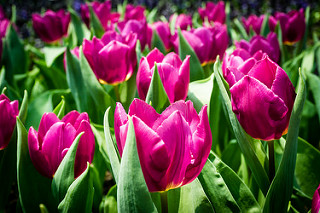
\includegraphics[width=0.8\textwidth]{images/1_1_tulips}
    \caption[Example of image classification]{Image classification: this image is classified as a tulip}
    \label{fig:figure-tulips}
\end{figure}
The object detection tasks consists of assigning a label and a bounding box to each object in the image.
The bounding box is a rectangle that encloses the object(\hyperref[fig:figure-object-detection]{Figure 1.2}).
\begin{figure}[H]
    \centering
    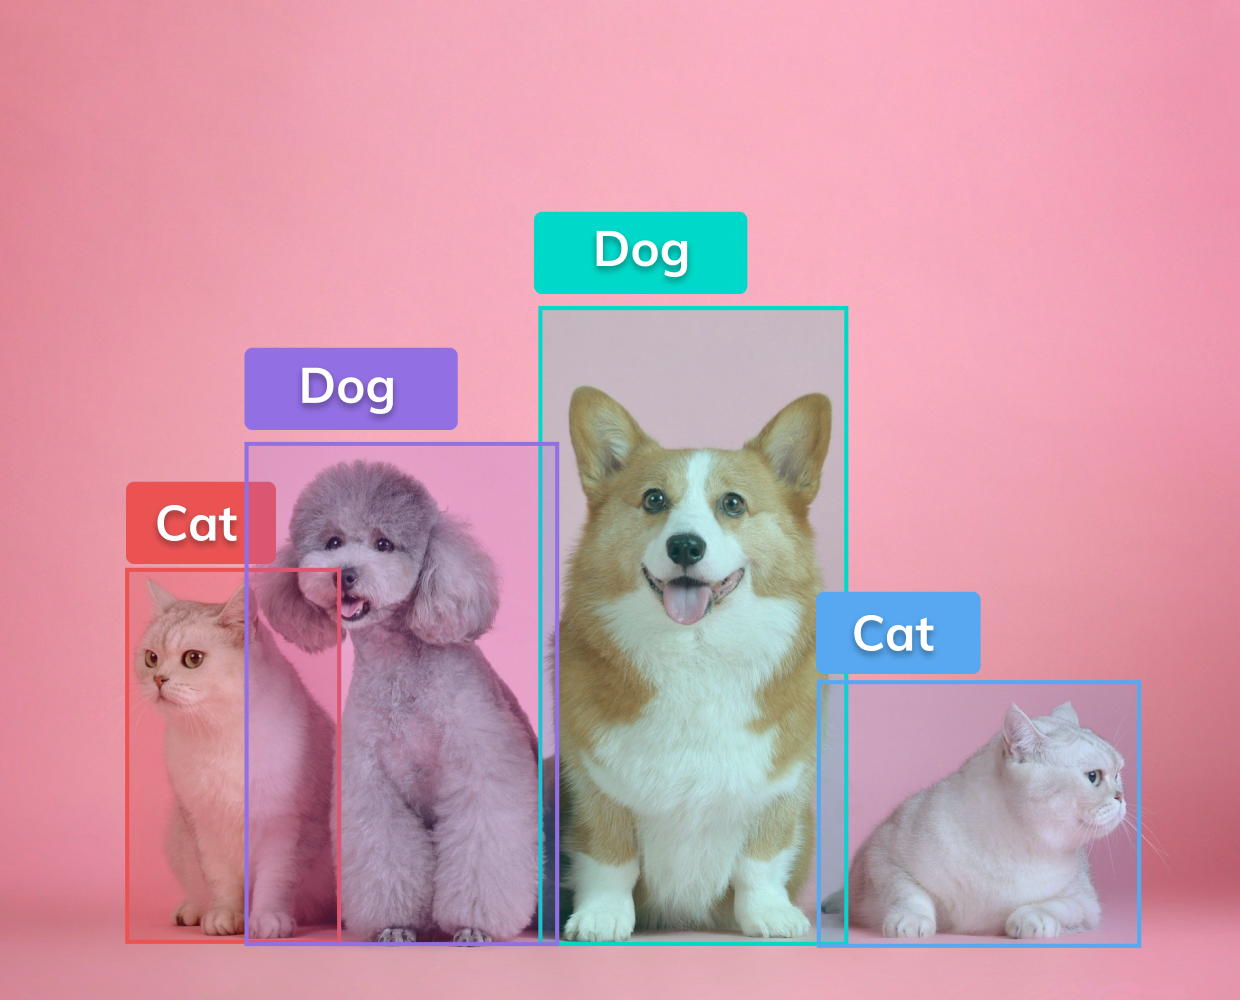
\includegraphics[width=0.8\textwidth]{images/1_1_object_detection}
    \caption[Example of object detection]{Object detection: this image contains two classes of objects, cat and dog.}
    \label{fig:figure-object-detection}
\end{figure}
The semantic segmentation task consists of assigning a label to each pixel of the image(\hyperref[fig:figure-semantic-segmentation]{Figure 1.3}).

\begin{figure}[H]
    \centering
    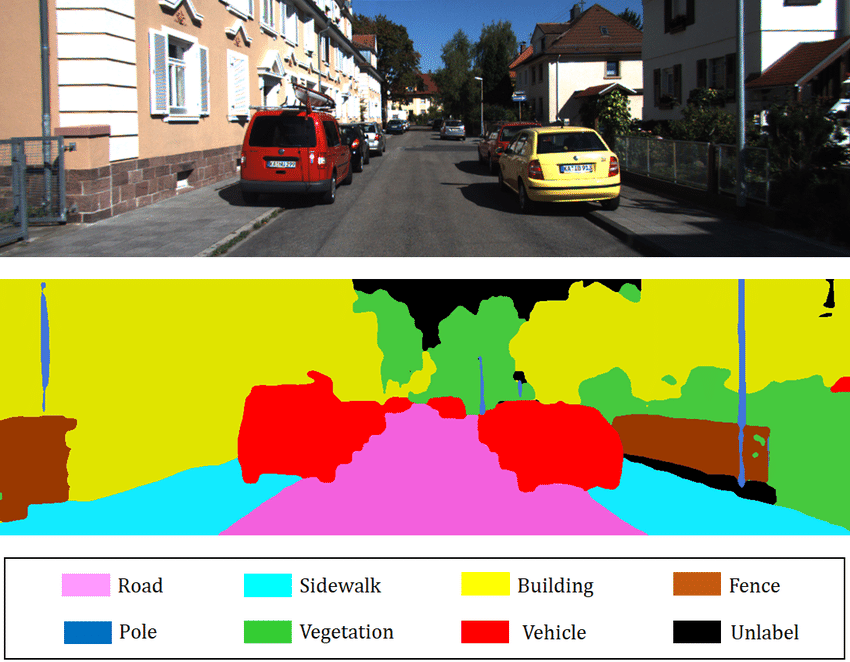
\includegraphics[width=0.8\textwidth]{images/1_1_semantic_segmentation}
    \caption[Example of semantic segmentation]{Semantic segmentation: each pixel is assigned a label.}
    \label{fig:figure-semantic-segmentation}
\end{figure}

Then, the modern CV systems can be used not only on the images, but also on video, like surveillance cameras to perform the real-time object detection and tracking, the most famous model is YOLOv3 (Redmon et al.~\cite{yolov3_paper}) (\hyperref[fig:figure-yolo-v3]{Figure 1.4}).

\begin{figure}[H]
    \centering
    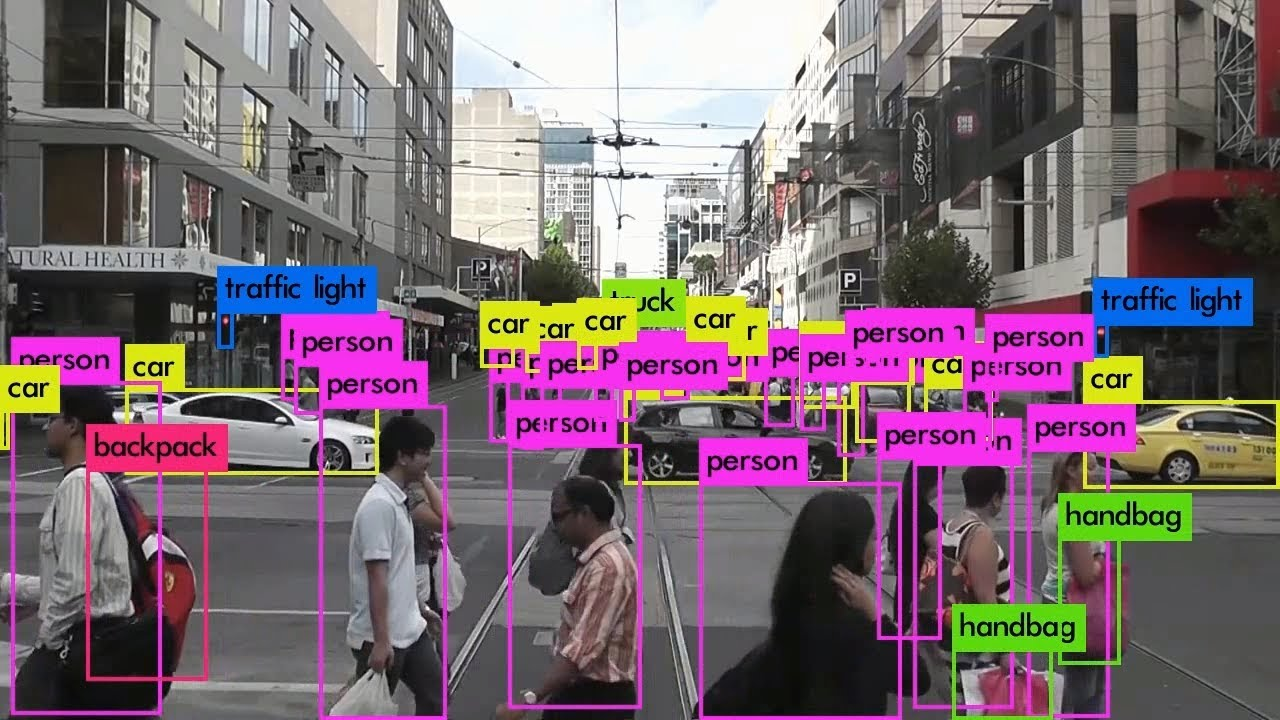
\includegraphics[width=0.8\textwidth]{images/1_1_yolov3}
    \caption{YOLO-V3 in action.}
    \label{fig:figure-yolo-v3}
\end{figure}



%**************************************************************

\section{Problem}\label{sec:problem}
The term "odometry" originated from two Greek works \emph{hodos} (meaning "journery" or "travel") and \emph{metron} (meaning "measure").
This derivation is related to the estimation of the change in a robot's pose (translation and rotation) over time.
Mobile robot use data from motion sensor to estimate their position relative to their initial location, this is called odometry.
VO is a technique used to localize a robot by using only a stream of images acquired from a single or multiple camera.
There are different ways to classify the typology of Visual Odometry:
\begin{itemize}
    \item based on the camera setup:
        \begin{itemize}
            \item Monocular VO: using only one camera;
            \item Stereo VO: using two cameras;
        \end{itemize}
    \item based on the information:
        \begin{itemize}
            \item Feature based method: which extracts the image feature points and tracks them in the image sequence;
            \item Direct method: a novel method which uses the pixel intensity in the image sequence directly as visual input.
            \item Hybrid method: which combines the two methods.
        \end{itemize}
    \item Visual inertial odometry: if a \gls{imu} is used within the VO system, it is commonly referred to as Visual inertial odometry.
\end{itemize}
We can represent the pose in different ways, for example: \textbf{euler angles}, \textbf{quaternions}, \textbf{rotation matrices} combined with \textbf{translation vectors}.

The goal is to create a \gls{nn}, using a \textbf{ResNet} to extract features from images and the \textbf{transformer} presented by Vaswani et al.~(\cite{transformer_paper}), which is able to estimate a sequence of camera poses given a sequence of images.

%**************************************************************

\section{Why transformer?}\label{sec:why-transformer}

We think that the transformer is a good candidate to solve the problem of visual odometry because it is able to learn a sequence from one domain and translate it into another sequence from another domain.
This kind of task is called sequence-to-sequence translation, e.g., machine translation.

Traditionally, this task is tackled by using recurrent neural networks (RNNs), but they have some limitations, such as the vanishing gradient problem, which makes them difficult to train.

Other VO approaches uses the CNNs, but in CNNs the features are statically weighted using pretrained weights, while in the transformer the features are dynamically weighted based on the context and receptive fields of CNNs can be limiting the performance of the whole network.
The success of the CNN derives from the fact the shared weights explicitly encode how specific identical patterns are repeated in images, this ensures the convergence also in relatively small dataset, but also limits the modelling capacity.
Meaning that CNNs can converge to a good performance also with a relatively small dataset.

Meanwhile, the vision transformers do not enforce such strict bias, so, transformer has the higher learning capacity, but it's harder to train.

So, given the high learning capacity of the transformer, its capability to adapt to various tasks and its good ability in seq2seq translation, we think that it is a good candidate to solve the problem of visual odometry.


%**************************************************************


\section{Solution}\label{sec:solution}
%**************************************************************
Researchers proposed special adversarial attacks in the text domain in order to maintain semantic consistency and syntactic correctness.
But those methods fail in generating high-quality adversarial examples since they frequently violate linguistic constraints.

This thesis concentrates on the adversarial attacks for text classification, in particular, the attacks based on sentiment analysis datasets, like IMDB \cite{maas-EtAl:2011:ACL-HLT2011} and Rotten Tomatoes \cite{pang-lee:2005a}.
Two state-of-the-art approaches, TextFooler \cite{journals/corr/abs-1907-11932} and BERT-based attack \cite{conf/emnlp/GargR20}, are compared to analyze weaknesses and strengths.

Then, their shortcomings are addressed by proposing a novel method, called SynBA, to generate adversarial examples for text data.
It is a word-level attack that generates adversarial examples by substituting words with candidates that have both a synonymy and contextual relationship with the original token.

The key contributions of this survey can be summarized as follows:
\begin{itemize}
    \item we introduce a simple but strong attack method, SynBA, to quickly generate high-profile utility-preserving adversarial examples that force the target models to make wrong predictions under the white-box setting;
    \item we propose a comprehensive automatic and human evaluation of adversarial attacks to evaluate the effectiveness, efficiency, and utility preserving properties of our system;
    \item we compare the adversarial examples generated by our method with TextFooler and BERT-based attack in terms of semantic similarity, semantic consistency, perturbation rate, success rate, perplexity and execution time.
\end{itemize}


% Our contributions. This survey concentrates on the adversarial
% attack and defense technology in the NLP field and provides a thorough and systematic review. 
%The key contributions of this survey
% can be summarized as follows:
%  We comprehensively and systematically summarize the textual
% adversarial attack and defense technology, elaborating on textual adversarial examples, adversarial attacks on texts, defenses
% against textual adversarial attacks, applications in various NLP
% tasks, and potential development directions in this domain.
%  We categorize current textual adversarial attacks according to
% the semantic granularity at the top level and further classify
% each class into several subclasses depending on the example
% generation strategy. To the best of our knowledge, we are the
% first to regard the example generation strategy as a classification criterion and propose this two-level classification for
% adversarial attacks.

%

% Briefly describe your methodology and/or theoretical approach
% Explain the aim of your research and what contribution it will make to the topic

% from TextFooler

% Our main contributions are summarized as follows:
% • We propose a simple but strong baseline, TEXTFOOLER, to quickly generate high-profile utility-preserving adversarial examples that force the target models to make wrong predictions under the black-box setting.
% • We evaluate TEXTFOOLER on three state-of-the-art deep learning models over five popular text classification tasks and two textual entailment tasks, and it achieved the state-of-the-art attack success rate and perturbation rate. Algorithm 1 Adversarial Attack by TEXTFOOLER
% • We propose a comprehensive four-way automatic and three-way human evaluation of language adversarial attacks to evaluate the effectiveness, efficiency, and utilitypreserving properties of our system.
% • We open-source the code, pre-trained target models, and test samples for the convenience of future benchmarking


%**************************************************************

\section{Thesis organization}\label{sec:thesis-organization}
\begin{description}
    \item[{\hyperref[ch:introduction]{First chapter}}] introduces the general content about thesis and gives a short presentation of the topic, the problem and the solution we propose;

    \item[{\hyperref[ch:background]{Second chapter}}] a deepening about the theoretical foundations used during the stage and the project;

    \item[{\hyperref[ch:methodology]{Third chapter}}] presents the datasets used during for the training and the testing of the model;

    \item[{\hyperref[ch:experimental-results]{Fourth chapter}}] presents the experiments did during to develop the system;

    \item[{\hyperref[ch:final-discussions]{Fifth chapter}}] discusses about the results and possible future developments.
\end{description}
During the drafting of the essay, following typography conventions are considered:
\begin{itemize}
    \item the acronyms, abbreviations, ambiguous terms or terms not in common use are defined in the glossary, in the end of the present document;
    \item the first occurrences of the terms in the glossary are highlighted like this: \gls{word};
    \item the terms from the foreign language or jargon are highlighted like this: \emph{italics}.
\end{itemize}

%**************************************************************


    % !TEX encoding = UTF-8
% !TEX TS-program = pdflatex
% !TEX root = ../tesi.tex

%**************************************************************

\chapter{Background}
\label{ch:background}
%**************************************************************

\intro{In this chapter we will present the theoretical knowledge useful to understand the content from successive chapters.}\\

%**************************************************************

\section{Natural Language Processing}\label{sec:nlp}
%**************************************************************

The field of \gls{nlp} %, also known as computational linguistics,
 is a branch of linguistics, computer science, and artificial intelligence focused on the technology of processing language.
It encompasses a variety of topics, which involves the engineering of computational models and
processes to solve practical problems in understanding and generating human
languages. These solutions are used to build useful software.

Linguistics has two
subfields---computational linguistics and theoretical linguistics. Computational
linguistics has been concerned with developing algorithms for handling a useful
range of natural language as input. While theoretical linguistics has focused
primarily on one aspect of language performance, grammatical competence---how
people accept some sentences as correctly following grammatical rules and others as ungrammatical. They are concerned with language universals—principles of
grammar which apply to all natural languages \cite{Cole:1996}.

Computational linguistics is concerned with the study of natural language analysis
and language generation. Further, language analysis is divided into two domains,
namely sentence analysis, and discourse and dialogue structure. Much more is known
about the processing of individual sentences than about the determination of discourse
structure. Any analysis of discourse structure requires a prerequisite as an analysis of
the meaning of individual sentences. However, it is a fact that for many applications,
thorough analysis of discourse is not mandatory, and the sentences can be understood
without that \cite{grishman_computational_1986}.

The sentence analysis is further divided into syntax analysis and semantic analysis.
The overall objective of sentence analysis is to determine what a sentence “means”.
In practice, this involves translating the natural language input into a language with
simple semantics, for example, formal logic, or into a database command language.
In most systems, the first stage is syntax analysis. Figure \ref*{fig:nlp_components} shows the relations
among different components of NLP \cite{Chowdhary2020}.

\begin{figure}[H]
    \centering
    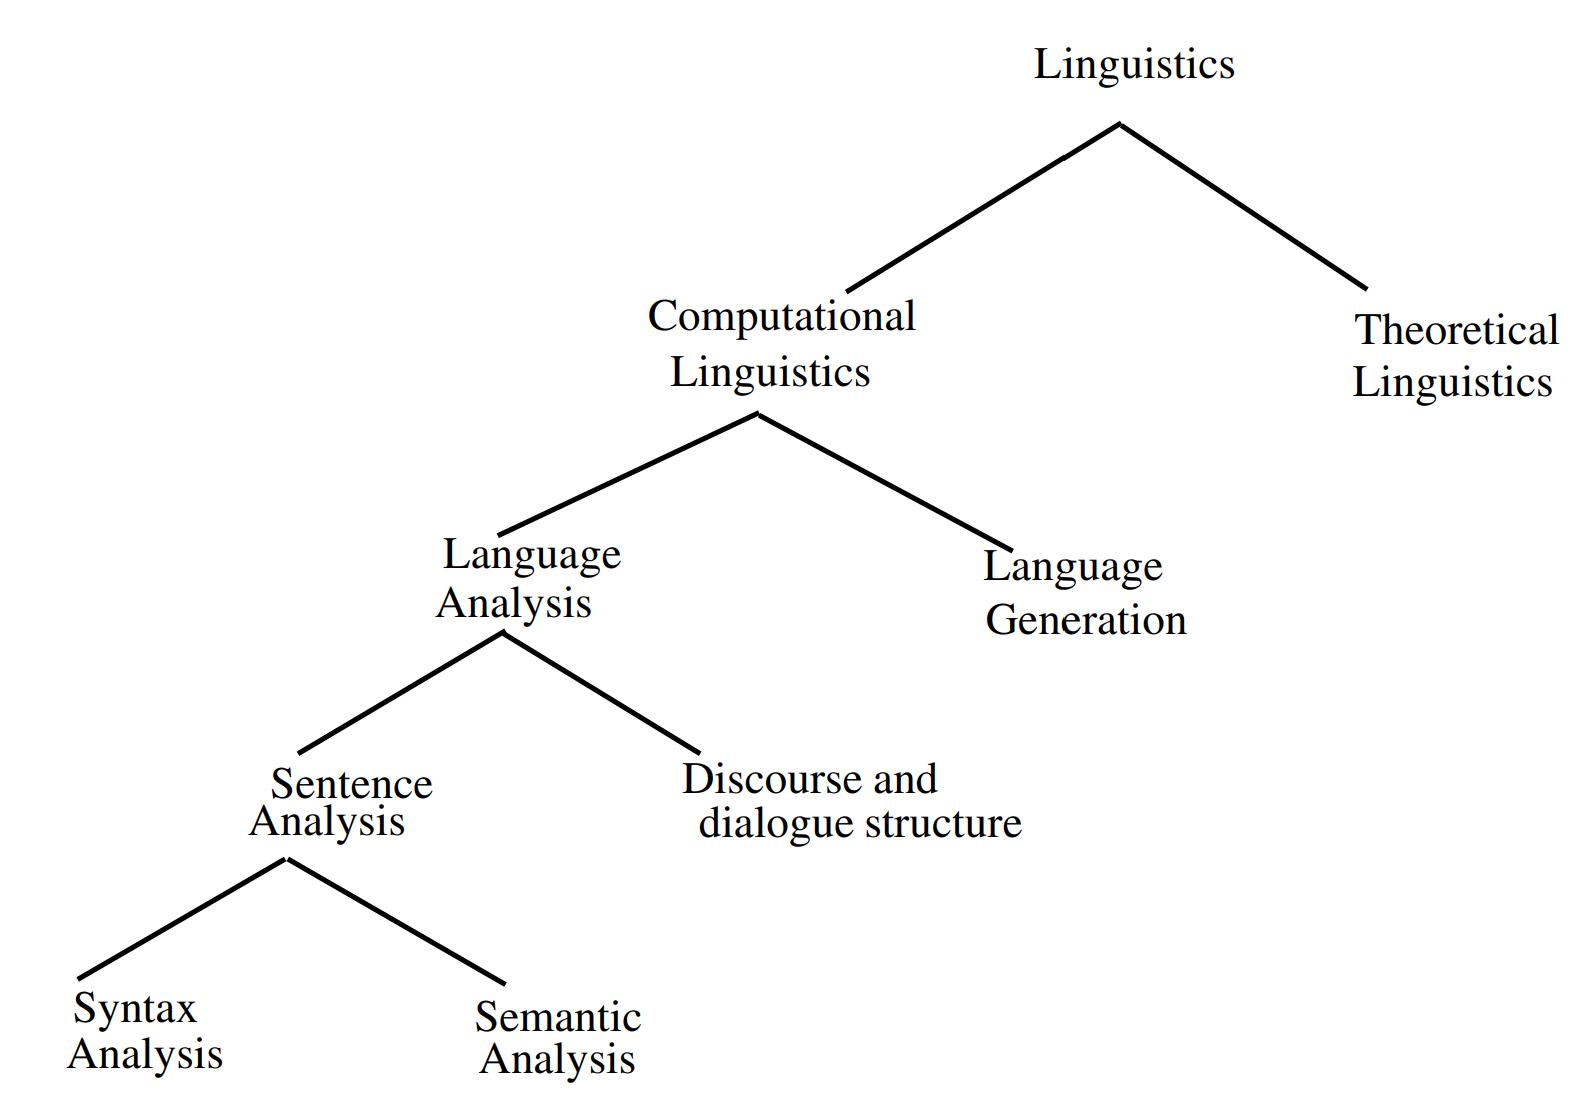
\includegraphics[width=0.8\textwidth]{images/2_1_nlp_components.png}
    \caption{Components of NLP}\label{fig:nlp_components}
\end{figure}
    

Some of the common applications of NLP are Classification of text into categories, Index and search large texts, Automatic translation, Information extraction,
Automatic summarization, Question answering, Knowledge acquisition, and Text
generations/dialogues.
Some of those tasks are discussed in sections \ref{subsec:text-classification}, \ref{subsec:sentiment-analysis}, \ref{subsec:nli}, \ref{subsec:seq2seq}.

%**************************************************************

\subsection{Lexicon}\label{subsec:lexicon}
Dictionaries are special texts whose subject matter is
a language, or a pair of languages in the case of a
bilingual dictionary. The purpose of dictionaries is to
provide a wide range of information about words---
etymology, pronunciation, stress, morphology, syntax, register---to give definitions of senses of words,
and, in so doing, to supply knowledge not just about
language, but about the world itself.

The term “dictionary” is typically related to printed wordbook for human readers. 
Instead “\gls{lexicon}” will refer to the component of
a NLP system that contains information (semantic,
grammatical) about individual word strings \cite{Guthrie_ComACM96}.

A lexicon which provides an effective combination of traditional
lexicographic information and modern computing is called WordNet \cite{miller1995wordnet}.
It is an online lexical database designed for use under program control. English nouns, verbs,
adjectives, and adverbs are organized into sets of synonyms, each representing
a lexicalized concept. WordNet contains more than 118,000 different word
forms and more than 90,000 different word senses. Approximately 40\% of
the words in WordNet have one or more synonyms.

The cognitive synonyms which are called \emph{synsets} are presented in the database with lexical and semantic relations. 
WordNet includes the following semantic relations:
\begin{itemize}
    \item \textbf{Hypernymy}: A hypernym is a word that is more general than the word in question. For example, a hypernym of “dog” is “canine”.
    \item \textbf{Hyponymy}: A hyponym is a word that is more specific than the word in question. For example, a hyponym of “dog” is “poodle”.
    \item \textbf{Synonymy}: A synonym is a word that has the same meaning as the word in question. For example, a synonym of “good” is “tasty”.
    \item \textbf{Antonymy}: An antonym is a word that has the opposite meaning of the word in question. For example, a antonym of “good” is “bad”.
\end{itemize}

%**************************************************************

\subsection{Word Embeddings}\label{subsec:word-embeddings}
The way machine learning models process data is different from how humans do. 
For example, we can easily understand the text “I saw a cat”, but our models can not --- they need vectors of features. 
Such vectors, called \glsplural{word embedding}, are representations of words which can be fed into a model.


\subsubsection{Word-count-based embedding}\label{subsubsec:bag-of-words}
A common approach to represent a text document is to use a column vector of word counts.
This embedding is often called a \gls{bag-of-words}, because it includes only information about the count of each word, and not the order in which the words appear.
The bag-of-words representation ignores grammar, sentence boundaries, paragraphs — everything but the words. Yet the bag of words model is surprisingly effective for text classification.

Another word-count-based method, widely used in the information retrieval, is \acrshort{tfidf}, short for term frequency-inverse document frequency, which aims to reflect the significance of the specified term in the document collection and is one of the most popular term weighting schemes.

\subsubsection{Dense embeddings}\label{subsubsec:static-embeddings}
Bag-of-words embeddings are sparse and long vectors with dimensions corresponding to words in the vocabulary or documents in a collection.
A more powerful word representation is a dense vector, where instead of mostly-zero counts, the values will be real-valued numbers that can be negative.
It turns out that dense vectors work better in every NLP task than sparse vectors.

Bengio et al. \cite{conf/nips/BengioDV00} presented a model which learned word representations using distributed
representation. The authors presented a neural model which obtains word representations as to
the product while training a \gls{language-model}.
The popularity of word representation methods are due to two famous models, Word2Vec
\cite{mikolov2013efficient} and GloVe \cite{pennington2014glove}.

\subsubsection{Contextual embeddings}\label{subsubsec:contextual-embeddings}
To address the issue of polysemous and the context-dependent nature of words, we need to
distinguish the semantics of words in different contexts.

Contextualised word embeddings are variable vectors that are dependent on the context in which the word is used.
So, representations of a given word are multiple and are
directly computed from their context. The context of a
word is usually composed of the words surrounding it.

These contextualized representations are set to the hidden states of a deep neural model, which is trained as a language model.
By running the language model, we obtain contextualized word representations, which can then be used as the base layer in a supervised neural network for any task. This approach yields significant gains over pre-trained word embeddings on several tasks, presumably because the contextualized embeddings use unlabeled data to learn how to integrate linguistic context into the base layer of the supervised neural network.


%**************************************************************

\subsection{Masked Language Models}\label{subsec:masked-language-models}
A \acrfull{mlm} is a pre-training technique which first masks out some tokens from the
input sentences and then trains the model to predict the masked
tokens by the rest of the tokens. A special \texttt{[MASK]} token is used to replace some words randomly in the original text.

Masked Language Modelling is usually solved as a classification problem. We feed the masked
sequences to a neural encoder whose output vectors are further fed into a softmax classifier to predict the masked token.

The most popular MLM is \acrshort{bert} \cite{devlin2018bert}, which is a bidirectional encoder representation from a particular deep learning architecture called \gls{transformer} \cite{vaswani2017attention}. 
It uses self-supervised training on the masked language modelling and next sentence prediction tasks to learn/produce contextual representations of words.

Concurrently, there are multiple research proposing different enhanced versions of MLM to further improve BERT. Instead
of static masking, RoBERTa \cite{liu2019roberta} improves BERT by dynamic masking.
While other models aim to optimize BERT's performance, DistilBERT \cite{sanh2019distilbert} has a different goal. Its target is to reduce the large size and enhance the speed of BERT while still keeping as much strength as possible.
DistilBERT reduces the size of $BERT_{BASE}$ by 40\%, enhances the speed by 60\% while retaining 97\% of its capabilities.
ALBERT \cite{lan2019albert} also reduces the model size of BERT and it does not have to trade-off the performance. Compared to DistilBERT, which uses BERT as the teacher for its distillation process, ALBERT is trained from scratch (just like BERT).

%**************************************************************
\subsection{Text classification}\label{subsec:text-classification}

Classification lies at the heart of both human and machine intelligence. Deciding what letter, word, or image has been presented to our senses, recognizing faces or voices, sorting mail, assigning grades to homeworks; these are all examples of assigning a category to an input.
In this section, we introduce text classification, the task of assigning a label or category to an entire text or document.

Given a text document, assign it a discrete label $y \in Y$, where $Y$ is the set of possible labels. 
Text classification has many applications, from spam filtering to the analysis of electronic health records, or the categorization of news articles.

Classification is essential for tasks below the level of the document as well.
An example of this is period disambiguation (deciding if a period is the end of a sentence or part of a word), or word tokenization (deciding if a character should be a word boundary). Even language modelling can be viewed as classification: each word can be thought of as a class, and so predicting the next word is classifying the context-so-far into a class for each next word. A part-of-speech tagger classifies each occurrence of a word in a sentence as, e.g., a noun or a verb.

The goal of classification is to take a single observation, extract some useful features, and thereby classify the observation into one of a set of discrete classes.

One method for classifying text is to use handwritten rules. There are many areas of language processing where handwritten rule-based classifiers constitute a state-of-the-art system, or at least part of it. Rules can be fragile, however, as situations or data change over time, and for
some tasks humans aren't necessarily good at coming up with rules. Most cases of classification in language processing are instead done via supervised machine learning, where an algorithm learns how to map from an observation to a correct output \cite{Jurafsky2009}.

Many kinds of machine learning algorithms are used to build classifiers.
Formerly, statistical and machine learning approaches, such as naïve Bayes, k-nearest neighbours, hidden Markov models, conditional random fields (CRFs), decision trees, random forests, and support vector machines, were widely used to design classifiers. 
However, during the past several years, there has been a wholesale transformation, and these approaches have been entirely replaced, or at least enhanced, by neural network models \cite{surveyNlpDeepLearning}. 

%**************************************************************
\subsection{Sentiment analysis}\label{subsec:sentiment-analysis}
A popular application of text classification is sentiment analysis, the extraction of sentiment, the positive or negative orientation that a writer expresses toward some object. A review of a movie, book, or product on the web expresses the author's sentiment toward the product, while an editorial or political text expresses sentiment toward a candidate or political action. Extracting consumer or public sentiment is thus relevant for fields from marketing to politics \cite{Jurafsky2009}.

The simplest version of sentiment analysis is a binary classification task, and
the words of the review provide excellent cues. Consider, for example, the following phrases extracted from positive and negative reviews of movies and restaurants. Words like great, richly, awesome, pathetic, awful and ridiculously are very informative cues:

\emph{$+$ ...zany characters and richly applied satire, and some great plot twists}
\par
\emph{$-$ It was pathetic. The worst part about it was the boxing scenes...}
\par
\emph{$+$ ...awesome caramel sauce and sweet toasty almonds. I love this place!}
\par
\emph{$-$ ...awful pizza and ridiculously overpriced...} 

The area of sentiment analysis it is becoming increasingly popular and utilizing deep learning. Applications are varied, including product research, futures prediction, social media analysis, and classification of spam \cite{ZhengWG18}. 
Good results were obtained using an ensemble, including both \acrshortpl{lstm} and \acrshortpl{cnn} \cite{Cliche17}.
But the current trend in state-of-the-art models in all application areas is to use pretrained stacks of transformer units in some configuration, whether in encoder-decoder configurations or just as encoders.

%**************************************************************

\subsection{Natural language inference}\label{subsec:nli}

The task of \acrfull{nli}, also
known as recognizing textual entailment,
asks a system to evaluate the relationships between
the truth-conditional meanings of two sentences
or, in other words, decide whether one sentence
follows from another.
The relationship can be entailment, contradiction, or neutral.

Specifically, natural language inference
is concerned with determining whether a natural language hypothesis \emph{h} can be inferred from a
premise \emph{p}, as depicted in the following example
from \cite{Manning2009NaturalLI}, where the hypothesis is
regarded to be entailed from the premise.

\emph{p: Several airlines polled saw costs grow more than
expected, even after adjusting}
\par
\emph{$\quad$ for inflation.}
\par
\emph{h: Some of the companies in the poll reported cost
increases.}


%**************************************************************

\subsection[Seq2Seq]{Sequence-to-Sequence models}\label{subsec:seq2seq}

All the tasks we have discussed so far are classification-based, where the input is a text and the output is a label. However, there are many tasks where the input and output are both sequences of tokens. 
For example, machine translation, summarization, and question answering are all tasks where we want to generate a sequence in human-like language as output.

A \acrfull{seq2seq} model is  is a special class of \acrfull{rnn} architectures  that can be used to solve these tasks.

In the general case, input sequences and output sequences have different lengths (e.g. machine translation) and the entire input sequence is required in order to start predicting the target. This requires a more advanced setup:
\begin{itemize}
    \item An \emph{encoder} processes the input sequence and returns its own internal state. This vector is called the context vector.
    \item A \emph{decoder} is a neural network that takes the context vector as input and outputs a sequence of tokens. It is trained to predict the next characters of the target sequence, given previous characters in the generated text. 
\end{itemize}


An example of this architecture is shown in Figure \ref{fig:seq2seq}.


\begin{figure}[h]
    \centering
    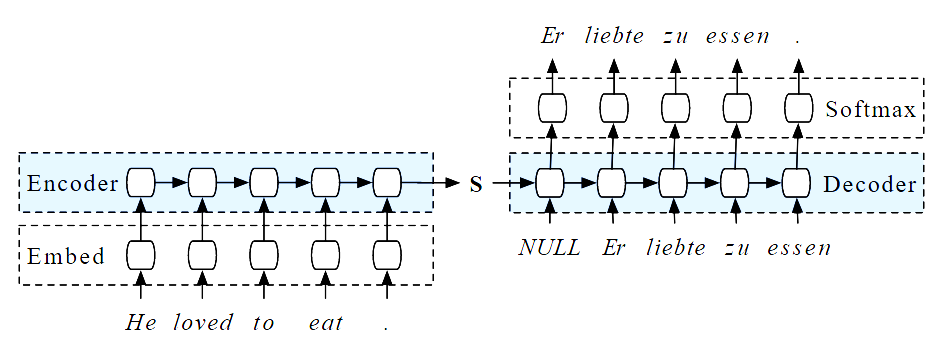
\includegraphics[width=0.8\linewidth]{images/2_1_seq2seq.png}
    \caption{An example of a sequence-to-sequence model for machine translation.}
    \label{fig:seq2seq}
\end{figure}

\vspace{1cm}

%**************************************************************


%**************************************************************

\section{Adversarial Machine Learning}\label{sec:adversarial-machine-learning}
Deep Learning algorithms have achieved the state-of-the-art performance in many tasks. 
However, the interpretability of deep neural networks is still unsatisfactory as they work as black boxes, which means it is difficult to get intuitions from what each neuron exactly has learned. 
One of the problems of the poor interpretability is evaluating the robustness of deep neural networks. 


Adversarial Machine Learning is a collection of techniques to train neural networks on how to spot intentionally misleading data or behaviors. 
This differs from the standard classification problem in machine learning, since the goal is not just to spot “bad” inputs, but preemptively locate vulnerabilities and craft more flexible learning algorithms.

The objective of an adversary
could be to attempt to manipulate either the data collection or
the data processing in order to corrupt the target model, thus
tampering the original output. 

Unlike traditional cybersecurity
attacks, these weaknesses are not due to mistakes made by programmers or users. They are
just shortcomings of the current state-of-the-art
methods. Put more bluntly, the algorithms that
cause AI systems to work so well are imperfect,
and their systematic limitations create opportunities for adversaries to attack. At least for the foreseeable future, this is just
a fact of mathematical life \cite{Comiter2019AttackingAI}.

Two main types of AI attacks can be defined according to the time at which the attack happens \cite{journals/corr/abs-1810-00069}:
\begin{itemize}
    \item \textbf{Adversarial Attacks (Evasion)}: this is the most common type of attack in
    the adversarial setting. The adversary tries to evade the system by adjusting malicious samples during testing phase. This
    setting does not assume any influence over the training data.
    In Figure \ref{fig:2_2_evasion} is depicted how adding an imperceptible and carefully constructed noise to the input originally regognized as “panda” with 57.7\% confidence, we can change
    the classification output given by the same neural network toward another target (in the example “gibbon” with 99.3\% confidence).
    \item \textbf{Data Poisoning Attacks}: This type of attack, known as contamination of the training data, is carried out at training phase of
    the machine learning model. An adversary tries to inject
    skilfully crafted samples to poison the system in order to
    compromise the entire learning process. The Figure \ref{fig:2_2_data_poisoning} shows as in normal machine learning (left), the learning algorithm extracts
    patterns from a dataset, and the “learned” knowledge is stored in the machine
    learning model---the brain of the system. In a poisoning attack (right), the
    attacker changes the training data to poison the learned model. 
\end{itemize}

\begin{figure}[H]
    \begin{subfigure}{0.45\textwidth}
      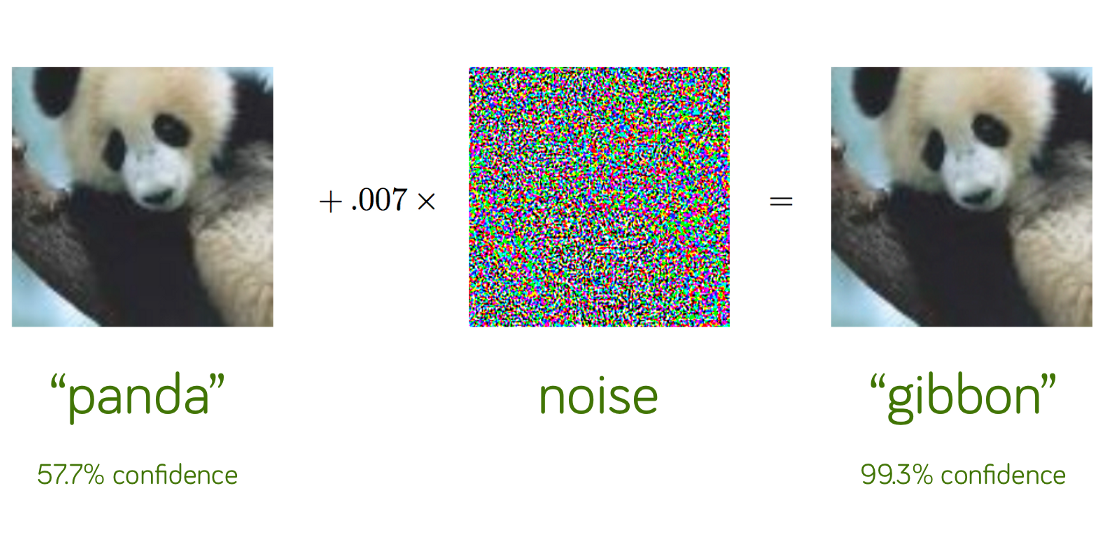
\includegraphics[width=\linewidth]{images/2_2_evasion.png}
      \caption{Evasion attack on image classification \cite{szegedy2013intriguing}} \label{fig:2_2_evasion}
    \end{subfigure}%
    \hspace*{\fill}   % maximize separation between the subfigures
    \begin{subfigure}{0.45\textwidth}
      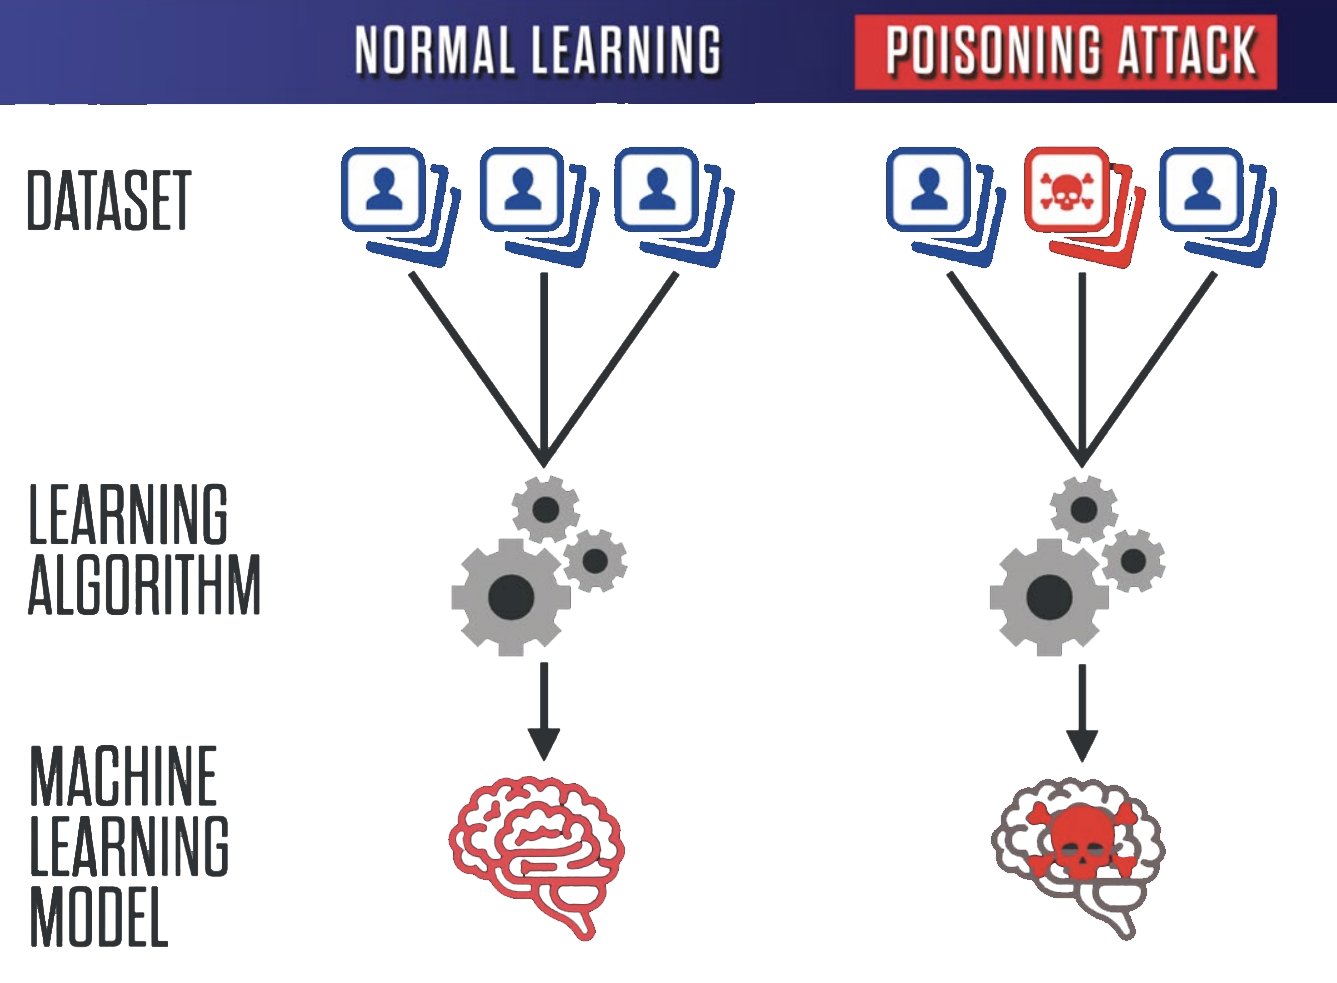
\includegraphics[width=\linewidth]{images/2_2_data_poisoning.png}
      \caption{Poisoning attack on training data \cite{Comiter2019AttackingAI}} \label{fig:2_2_data_poisoning}
    \end{subfigure}
  \caption{Examples of Artificial Intelligence Attacks} \label{fig:2_2_adversarial_attacks}
  \end{figure}

In this thesis, we will focus on the first type of attack, the Adversarial Attacks.
Over past few years, researchers \cite{goodfellow2014explaining, szegedy2013intriguing} used small unperceivable perturbations to evaluate the robustness of deep neural networks and found that they are not robust to these perturbations. 

%**************************************************************
\subsection{Adversarial examples}\label{subsec:adversarial-attacks}

Szegedy et al. \cite{szegedy2013intriguing} first evaluated the state-of-the-art deep neural networks used for image classification with small generated perturbations on the input images.
They found that the image classifiers were fooled with high probability, but human judgment is not affected. The perturbed image pixels were named \emph{adversarial examples} and this notation is later used to denote all kinds of perturbed samples in a general manner.
Formally, adversarial example $x^\prime$ is an example created via worst-case perturbation of the input to a deep learning model. An ideal deep neural network would still assign correct class $y$ (in the case of classification task) to $x^\prime$, 
while a victim deep neural network would have high confidence on wrong prediction of $x^\prime$. $x^\prime$ can be formalized as:
\begin{equation}
    \begin{array}{l}
    x^\prime = x + \eta, \quad f(x)=y, \quad x \in X,\\
    f(x^\prime) \neq y, \\
    \text{or} \quad f(x^\prime) = y^\prime, \quad y \neq y^\prime
    \end{array}
\end{equation}
where $\eta$ is the worst-case perturbation. The goal of the adversarial attack can be deviating the label to incorrect one ($f(x^\prime) \neq y$) or specified one ($f(x^\prime) = y^\prime$) \cite{journals/tist/ZhangSAL20}.

%**************************************************************
\subsection[Paradigm shift]{Paradigm shift: from CV to NLP}\label{subsec:paradigm-shift}
Adversarial examples were first proposed for attacking DNNs for object recognition in the \acrfull{cv} community.
The former work on this field by Szegedy et. al. \cite{szegedy2013intriguing}  was based on L-BFGS, but despite the effectiveness of the method, it was computationally expensive and impractical.
Goodfellow et al. \cite{goodfellow2014explaining} proposed a \acrfull{fsgm} that popularized this research topic. It is a simplification of the L-BFGS method since it add a small perturbation to the input of a model, which is computed by taking the sign of the gradient of the loss function with respect to the input.
Most follow-up research was based on optimizaion methods (eg. JSMA \cite{journals/corr/PapernotMJFCS15}, DeepFool \cite{journals/corr/Moosavi-Dezfooli15}, C\&W \cite{journals/corr/CarliniW16a}) or leveraging \acrfull{gan} to generate adversaries \cite{journals/corr/abs-1710-11342}.

As shown in Figure \ref{fig:2_2_adversarial_trend}, adversarial technology has attracted attention and has developed rapidly. Based on the paper list\footnote{\url{https://nicholas.carlini.com/writing/2019/all-adversarial-example-papers.html}} collected by Carlini, the chart counts
the number of publications related to adversarial in the CV and NLP fields. Compared with studies in the CV field, the publications in the NLP domain are far less. However, due to the wide application of NLP technology in text classification, sentiment analysis, text question-answering, neural machine translation, text generation and other tasks, as well as the continuous deepening of adversarial attack and defense technologies, the textual adversarial technology has gradually gained researchers' attention.

\begin{figure}
    \centering
    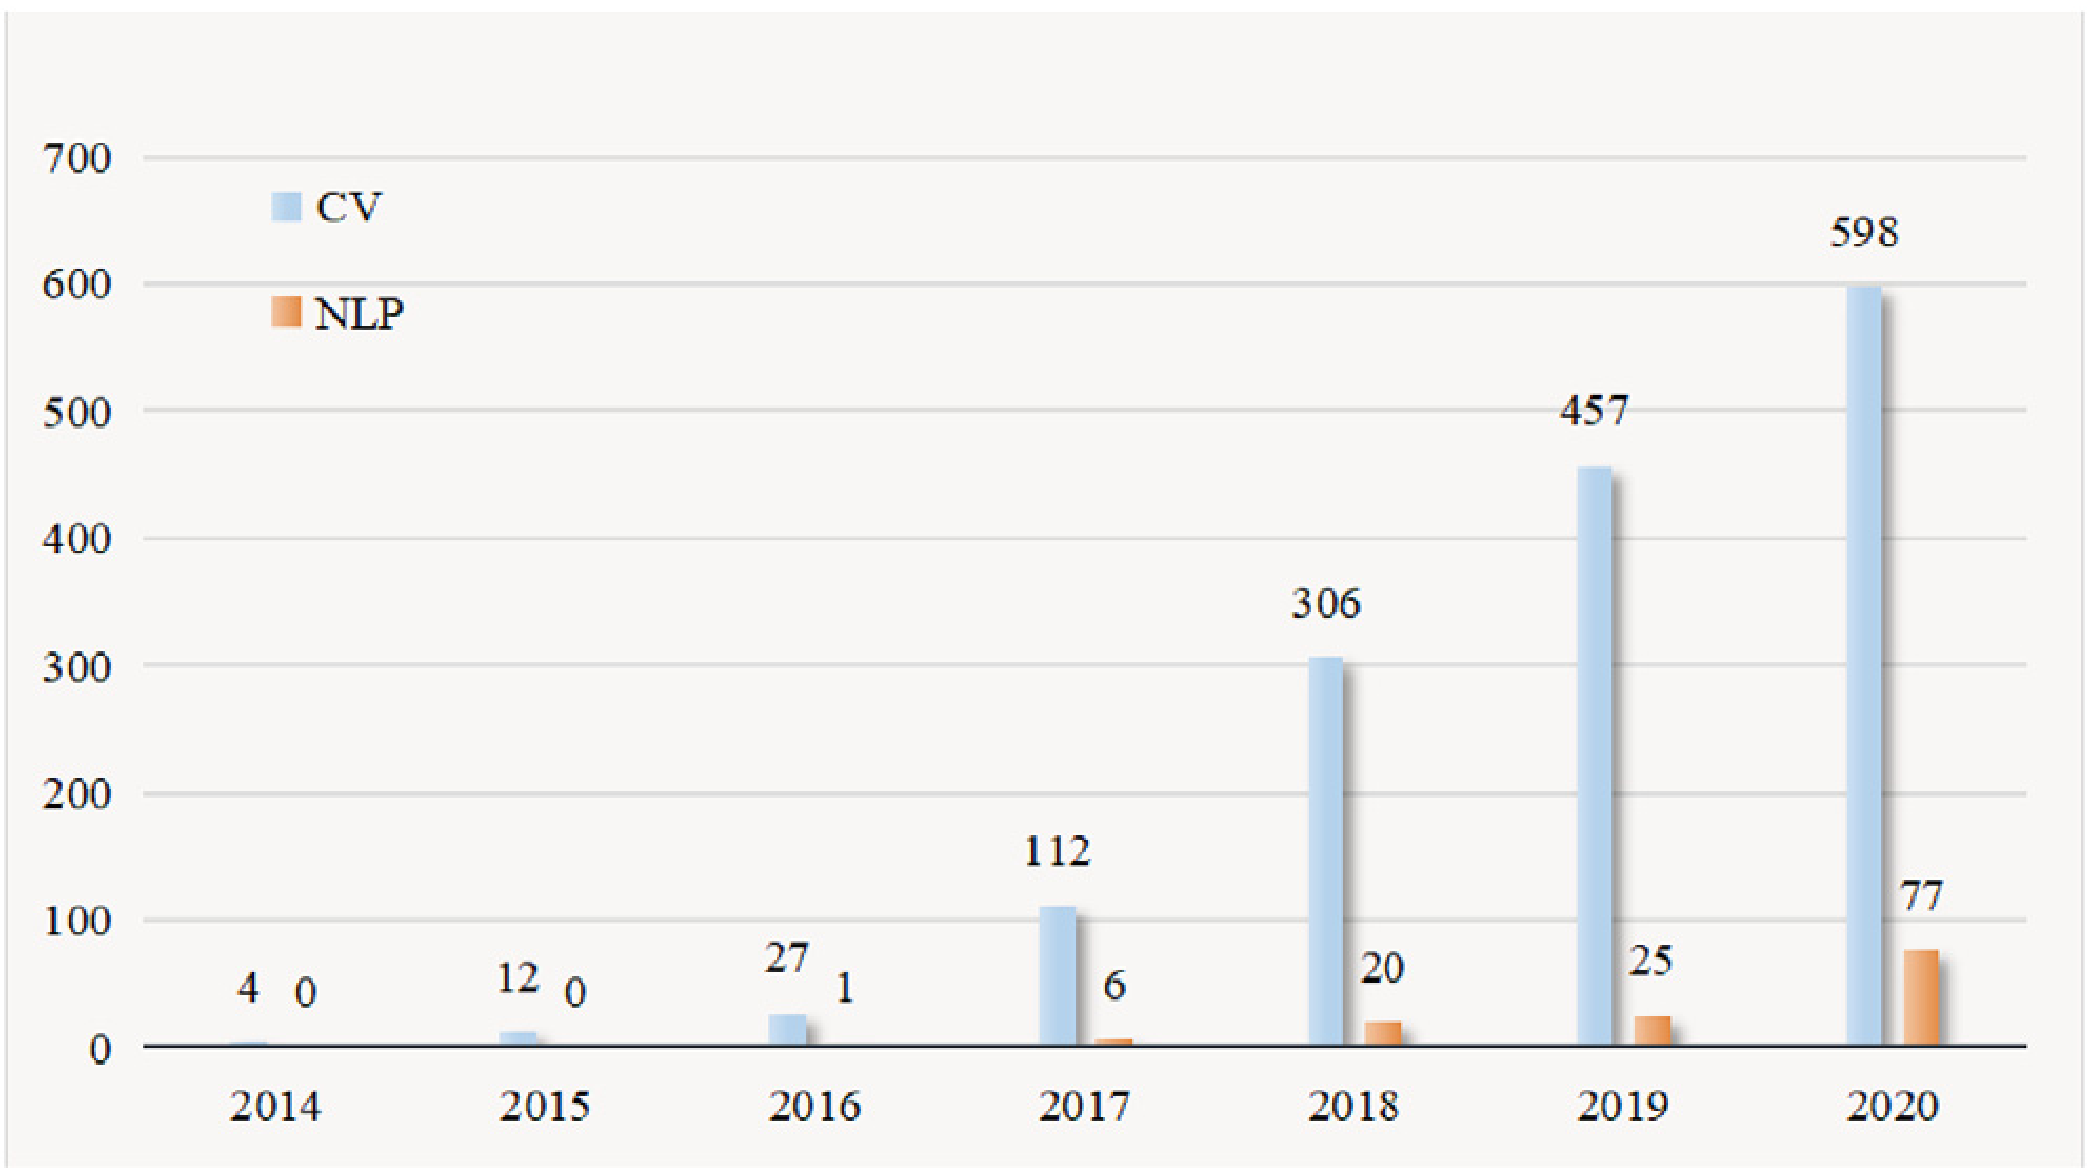
\includegraphics[width=0.8\linewidth]{images/2_2_papers.png}
    \caption{Adversarial technology trend in CV and NLP fields \cite{QIU2022278}}
    \label{fig:2_2_adversarial_trend}
\end{figure}

Papernot et al. \cite{journals/corr/PapernotMSH16} is the first to investigate adversarial attacks
on texts. Inspired by the idea of generating adversarial images, they crafted adversarial texts through the forward derivative associated with texts' embeddings, by modifying characters or words in original texts.


\subsubsection{Particularities of adversarial text}\label{subsubsec:particularities-of-adversarial-text}

Publications related to adversarial technology in the NLP field are far less than those in the CV field.
The reason is that three extra constraints need to be considered when generating textual adversarial examples. Specifically:
\begin{itemize}
    \item \textbf{Discrete}: Unlike images represented by continuous pixel values, the symbolic text is discrete. Therefore, finding appropriate perturbations is critical to efficient textual adversarial example generation. 
                             It is hard to define the perturbations on texts. Carefully designed variants or distance measurements for textual perturbations are required.
    \item \textbf{Perceivable}: The well-performed adversarial image generation method is based on the premise that a few pixel value changes in an image are invisible to human eyes. However, a slight modification of a character or word is easily realized by human eyes and spelling checkers. Hence, finding textual adversarial examples that are hard to be observed by human eyes is vital for successful adversarial attacks.
    \item \textbf{Semantic}: Compared with images whose overall semantics do not change when changing a few pixel values, the semantics of a text could be altered by even replacing or adding a character, violating the principle that adversarial examples are perceivable to humans. Therefore, keeping the semantics consistent is the key to crafting influential adversarial texts.
\end{itemize}

These differences make it extraordinarily difficult for
researchers to employ methods dealing with images to adversarial attacks. Moreover, one of the first tasks of NLP
models is to work on real data to check their generalization ability. Although adversarial attacks are a practical approach to evaluate robustness, most of them have the problem of being task-specific, not being well generalized, and not presenting comprehensive guidelines for evaluating system robustness.

%**************************************************************
\subsection{Taxonomy of textual adversarial attacks}\label{subsec:taxonomy-textual-adversarial-attacks}

Textual adversarial attack methods can be categorized according different criteria. In this section, we will introduce the taxonomy of textual adversarial attacks based on model access, adversarial goal, semantic granularity and attack strategy, as shown in Figure \ref{fig:2_2_taxonomy}.

\begin{figure}
    \centering
    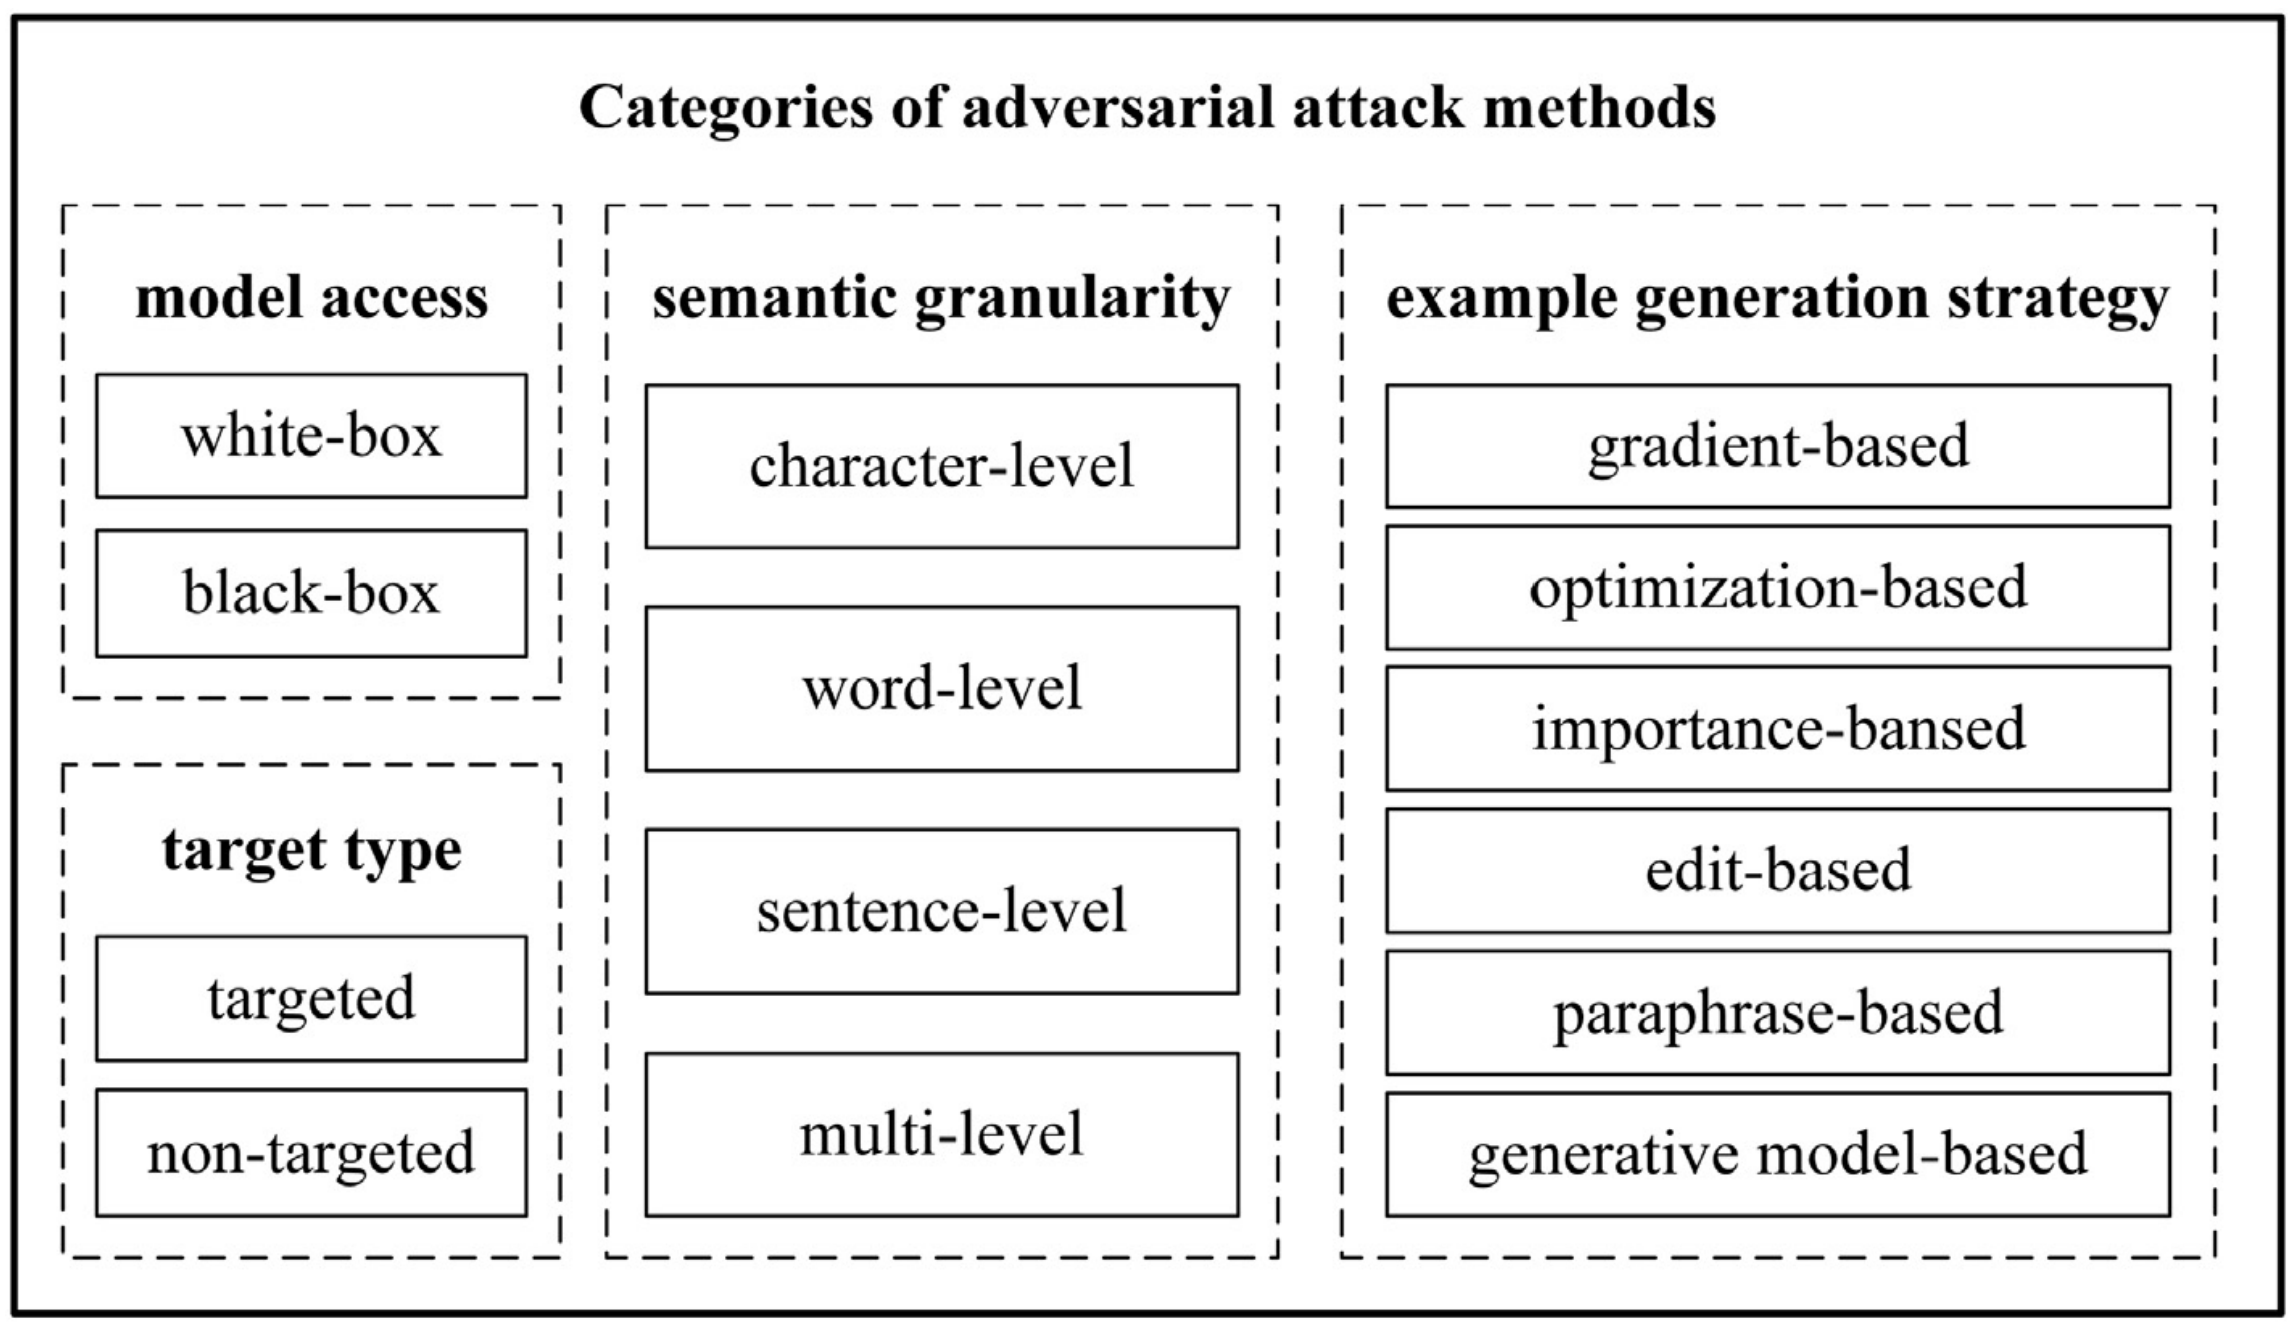
\includegraphics[width=0.8\linewidth]{images/2_2_taxonomy.png}
    \caption{Categorization of textual adversarial attack methods \cite{QIU2022278}}
    \label{fig:2_2_taxonomy}
\end{figure}

%-------------------------------------------------------------
\subsubsection{Model access}\label{subsubsec:model-access}

Adversarial attacks at the testing time do not tamper with the targeted model but rather forces it to produce incorrect outputs. 
The effectiveness of such attacks
is determined mainly by the amount of information available to the adversary about the model.
Testing phase attacks can be broadly classified into either \emph{white-box} or \emph{black-box} attacks \cite{journals/corr/abs-1810-00069}.

\textbf{White-Box Attacks}. In white-box attack on a machine learning model, an adversary has total
knowledge about the model used for classification (e.g., type of neural network along with number of layers). The attacker has information about the algorithm used in training (e.g.
gradient-descent optimization) and can access the training data distribution. He also knows the
parameters of the fully trained model architecture. The adversary utilizes available information
to identify the feature space where the model may be vulnerable, for which the model has
a high error rate. Then the model is exploited by altering an input using adversarial example
crafting method.

\textbf{Black-Box Attacks}. Black-box attack, on the contrary, assumes no knowledge about the model
and uses information about the settings or past inputs to analyse the vulnerability of the model.
For example, in an oracle attack, the adversary exploits a model by providing a series of carefully
crafted inputs and observing outputs.  For example, to identify meaningful words in given texts, works in \cite{journals/corr/SamantaM17, conf/acl/RenDHC19, journals/corr/abs-1907-11932} computed the probability change value, word saliency, and classification probability by using the victim model's output.


%-------------------------------------------------------------
\subsubsection{Adversarial goal}\label{subsubsec:adversarial-goal}

According to the attack purpose of an adversary, adversarial
attack methods are categorized into targeted and non-targeted attacks \cite{QIU2022278}.

\textbf{Non-targeted attack}. The adversary hopes to generate an adversarial example $x^\prime$ that makes the victim model $f$ produce a wrong output $f(x^\prime) \neq y$, where $y$ is the correct label of the input $x$. Since there is no limit on the target wrong output, this kind of attack is more frequently employed.

\textbf{Targeted attack}. In this scenario, the adversary intends to generate adversarial examples that make victim models output a specified wrong prediction. More specifically, the adversary hopes that the generated example $x^\prime$ to cause the victim model $f$ outputting $t=f(x^\prime)$, where $t$ is the output specified by the adversary.

%-------------------------------------------------------------
\subsubsection{Attack strategy}\label{subsubsec:attack-strategy}

According to different strategies in the adversarial example generation process, Shilin Qiu et al. \cite{QIU2022278} divide adversarial attacks into six types: gradient-based, optimization-based, importance-based, editbased, paraphrase-based, and generative model-based methods. Among them, strategies like the gradient-based method are evolved from adversarial image generation methods, and the implementation process of these attacks is usually relatively straightforward. While other methods like the optimizationbased and edit-based methods are proposed for discrete data, they generally show better performance in maintaining semantic consistency and grammatical correctness; however, they have enormous difficulty when designing well-turned algorithms.

\textbf{Gradient-based}. These methods calculate the forward derivative to the input and obtain adversarial perturbations by gradient backpropagation. Therefore, the vectorization for text needs to be implemented at first.

\textbf{Optimization-based}. It regards the adversarial example generation as a minimax optimization problem, i.e., maximizing the victim model's prediction error while the difference between the adversarial example and the original one is within an acceptable range. Currently, researchers craft adversarial texts essentially based on evolutionary algorithms, such as the \acrshort{ga} and \acrshort{pso}.

\textbf{Importance-based}. This means that which object is to be modified and how to modify it are determined by each object's importance related to the victim model. Since the more critical the changed word is, the easier it is to change the prediction of the victim model, even if the change is small enough. The adversarial example generated by this strategy generally maintains semantic consistency, grammatical, and syntactic correctness well.

\textbf{Edit-based}. It crafts adversarial examples by operations like inserting, removing, and swapping characters, words, or sentences. These editing operations are also used in other approaches, such as gradient-based, optimization-based, and importance-based methods. Therefore, the edit-based method refers to attacks that utilize the above editing operations but do not use the gradient information, optimization algorithm, or item importance.

\textbf{Paraphrase-based}. The adversary takes the paraphrase of a sentence as its adversarial example. In the paraphrase generation process, the adversary introduces different extra conditions to fool the victim model without affecting human judgment. The sentence-level attacks commonly use these approaches.

\textbf{Generative model-based}. This method uses the generative model like the GAN and encoder-decoder model to generate adversarial texts, and is frequently used in sentence-level attacks. Since there are gradient back propagations when training the generative model or crafting adversarial examples, these methods are usually combined with other techniques, such as \acrshort{rl}.

%-------------------------------------------------------------
\subsubsection{Semantic granularity}\label{subsubsec:semantic-granularity}

Since the text is discrete, classifying adversarial attacks according to semantic granularity is more intuitive than NLP tasks or black/white-box scenarios.
Thus, Huq et al. \cite{https://doi.org/10.48550/arxiv.2005.14108} divided textual adversarial attacks into four categories: the character-level, word-level, sentencelevel, and multi-level attack.

\textbf{Character-Level Attack}. Individual characters in this attack are either modified with new characters, special characters, and numbers. These are either added to the texted, swapped with a neighbor, removed from the word, or flipped.

\textbf{Word-Level Attack}. In this attacks words from the texts are changed with their synonyms, antonyms, or changed to appear as a typing mistake or removed completely.

\textbf{Sentence-Level Attack}. This attack inserts extra distractor sentences, generates the paraphrase, or modifies the original sentence structure to fool the victim model.

\textbf{Multi-Level Attack}. Attacks which can be used in a combination of character, word, and sentence level are called multi-level attack.

%**************************************************************
\subsection{Adversarial attack methods from literature}\label{subsec:aam-from-literature}

Several adversarial attack methods have been proposed in the literature. In this section, we present a brief overview of the most popular ones, listed in Table \ref{tab:attack-methods}.

Those methods are categorized according to the classification defined in Sec. \ref{subsubsec:semantic-granularity}:
1 character-level attack (DeepWordBug \cite{journals/corr/abs-1801-04354}), 4 word-level attacks (Probabilistic Weighted Word Saliency (PWWS) \cite{conf/acl/RenDHC19}, TextFooler \cite{journals/corr/abs-1907-11932}, BERT-based attack \cite{conf/emnlp/LiMGXQ20} and Semese-PSO \cite{conf/acl/ZangQYLZLS20}), 2 sentence-level attacks (Synthetically Controlled Paraphrase Networks (SCPNs \cite{conf/naacl/IyyerWGZ18}), and GAN-based attack \cite{journals/corr/abs-1710-11342}), and 1 multi-level attack (TextBugger \cite{conf/ndss/LiJDLW19}).

DeepWordBug detemines top critical tokens and modifies them by character-level transformations introducing typos. 
PWWS is a synonym substitution method that make use of the word saliency and classification probability.
TextFooler identifies important words, and replace them with the most semantically similar and grammatically correct substitutes.
BERT-based attack finds the vulnerable words for the target model and replaces them with candidates from a pre-trained BERT model.
Semese-PSO reduces search space by a sememe-based word replacement method, searching for adversarial examples by the PSO algorithm in the reduced search space.
SCPNs generates adversarial examples by paraphrasing the original sentence using an encoder-decoder model.
GAN-based attack generates adversarial examples using iterative stochastic search and hybrid shrinking search. The framework consisting of a GAN and a converter.
TextBugger generates character-level and word-level adversarial texts according to the importance in black-box and white-box scenarios.



\begin{table}[h]
  \footnotesize
  \centering
  \begin{tabular}{|l||l|l|l|l|}
    \hline
    Method & Granularity & Strategy & Model access & Attack goal \\
    \hline \hline
    DeepWordBug & Character-level & Importance-based & Black-box & Non-targeted \\ 
    \hline
    PWWS & Word-level & Importance-based & Black-box & Non-targeted \\
    \hline
    TextFooler & Word-level & Importance-based & Black-box & Non-targeted \\
    \hline
    BERT-based & Word-level & Importance-based & Black-box & Non-targeted \\
    \hline
    Semese-PSO & Word-level & Optimization-based & Black-box & Non-targeted \\
    \hline
    SCPNs & Sentence-level & Paraphrase-based & Black-box & Non-targeted \\
    \hline
    GAN-based & Sentence-level & Generative model-based & Black-box & Non-targeted \\
    \hline
    TextBugger & Multi-level & Importance-based & Black/White-box & Non-targeted \\
    \hline
  \end{tabular}
  \caption{Several adversarial attack methods from literature}
\label{tab:attack-methods}
\end{table}

%--------------------------------------------------------------
\subsubsection{TextFooler}\label{subsubsec:textfooler}

%--------------------------------------------------------------
\subsubsection{BERT-based attacks}\label{subsubsec:bert-based-attacks}

%**************************************************************

\section{Machine Learning hardening}\label{sec:ml-hardening}
%**************************************************************
Adversarial examples demonstrate that many modern machine learning algorithms can be broken easily in surprising ways. 
An essential purpose for generating adversarial examples for neural networks is to utilize these adversarial examples to enhance the model's robustness.

The overwhelming amount of work in the last few years for adversarial defenses has given good competition to the novel adversarial attack algorithms and considerably improved the robustness of existing deep learning models. These defense mechanisms are also used as regularization techniques to avoid overfitting, and making the model more robust \cite{https://doi.org/10.48550/arxiv.2203.06414}.

%**************************************************************
\subsection{Vanilla adversarial training}\label{subsec:adversarial-training}
One of the most popular adversarial defence approach is adversarial training.
It was first introduced in the work proposed in \cite{goodfellow2014explaining}. 
It is a method of defending against adversarial attacks by introducing adversarial examples in the training data. 
The strength of adversarial examples decides the final robustness and generalization achieved by the model.

This method can be seen as a data augmentation mechanism that extends the original training set with the successfully generated adversarial examples and try to let the model see more data during the training process.
Adversarial examples need to be carefully designed when training on adversarial examples to improve the model.

Although adversarial training can effectively improve the robustness of NLP models, this approach has some problems: 
\begin{itemize}
    \item extensive adversarial examples need to be prepared in advance, resulting in a massive calculation consumption
    \item it is likely to reduce the model classification accuracy
\end{itemize}

%**************************************************************
\subsection{Attack to Training}\label{subsec:a2t}
High computational cost hinders the use of vanilla adversarial training in NLP, and it is unclear how and as to what extent such training can improve an NLP model's performance.

Yoo et al. \cite{https://doi.org/10.48550/arxiv.2109.00544} propose to improve the vanilla
adversarial training in NLP with a computationally cheaper adversary, referred to as \acrfull{a2t}. 
A2T attempts to generate adversarial examples on the fly during training of the model on the training set, which is much cheaper than generating adversarial examples in advance.
This approach can improve an NLP model's robustness to the attack it was originally trained with and also defend the model against other types of word substitution attacks.

The attack component in A2T is designed to be is faster than previous attacks from literature. Previous attacks such as \cite{conf/emnlp/GargR20, journals/corr/abs-1907-11932} iteratively replace one word at a time to generate adversarial examples.
One issue with this method is that an additional
forward pass of the model must be made for each.
word to calculate its importance. For longer text inputs, this can mean that we have to make up to hundreds of forward passes to generate one adversarial example.

A2T instead determines each word's importance
using the gradient of the loss. For an input text including $n$ words: $x = (x_1, x_2, . . . , x_n)$ where each $x_i$ is a word, the importance of $x_i$ is calculated as:
\begin{equation}
    I(x_i) = \| \nabla_{e_i} L(\theta, x, y) \|_1
\end{equation}

where $e_i$ is the word embedding that corresponds to word $x_i$. For BERT and RoBERTa models where inputs are tokenized into sub-words, we calculate the importance of each word by taking the average of all sub-words constituting the word. This requires only one forward and backward
pass and saves us from having to make additional forward passes for each word.


%**************************************************************

\section{Text Attack}\label{sec:text-attack}
%**************************************************************

%**************************************************************
\subsection{Framework structure}\label{subsec:framework-structure}

%**************************************************************
\subsection{Attack components}\label{subsec:attack-components}

%**************************************************************
\subsection{HuggingFace integration}\label{subsec:huggingface-integration}

%**************************************************************
    % !TEX encoding = UTF-8
% !TEX TS-program = pdflatex
% !TEX root = ../tesi.tex

%**************************************************************
\chapter{Methodology}
\label{ch:methodology}
%\intro{In this chapter we will present the datasets created and used for the visual odometry.}

% - Introduction\\
% - Research Design\\
% - Research Questions and Hypotheses\\
% - Setting and Sample\\
% - Data Collection\\
% - Data Analysis\\
% - Conclusion\\


% demonstration of fit between methods chosen and research question(s)
% rationale for choosing materials, methods and procedures
% details of materials, equipment and procedures that will allow others to:
% replicate experiments
% understand and implement technical solutions

%**************************************************************

\section{Defined goal}\label{sec:defined-goal}
%**************************************************************

Most recent adversarial attack methods described in \ref{subsec:taxonomy-textual-adversarial-attacks} successfully decrease the accuracy of the target model.
However, since the main goal of the research is to enhance the robustness of the target model, we need to ensure that the quality of the crafted adversarial examples should be high, because the target model will be re-trained with them.

A successful natural language adversarial example can be defined as a perturbation that fools the model and fulfils  a set of linguistic constraints.
As an example in sentiment analysis (Figure \ref{fig:3_adverarial_example}), an attacker can fool the system by changing only one word from “Perfect” to “Spotless,” which can completely change the predicted output without being discerned by humans.

\begin{figure}[h]
    \centering
    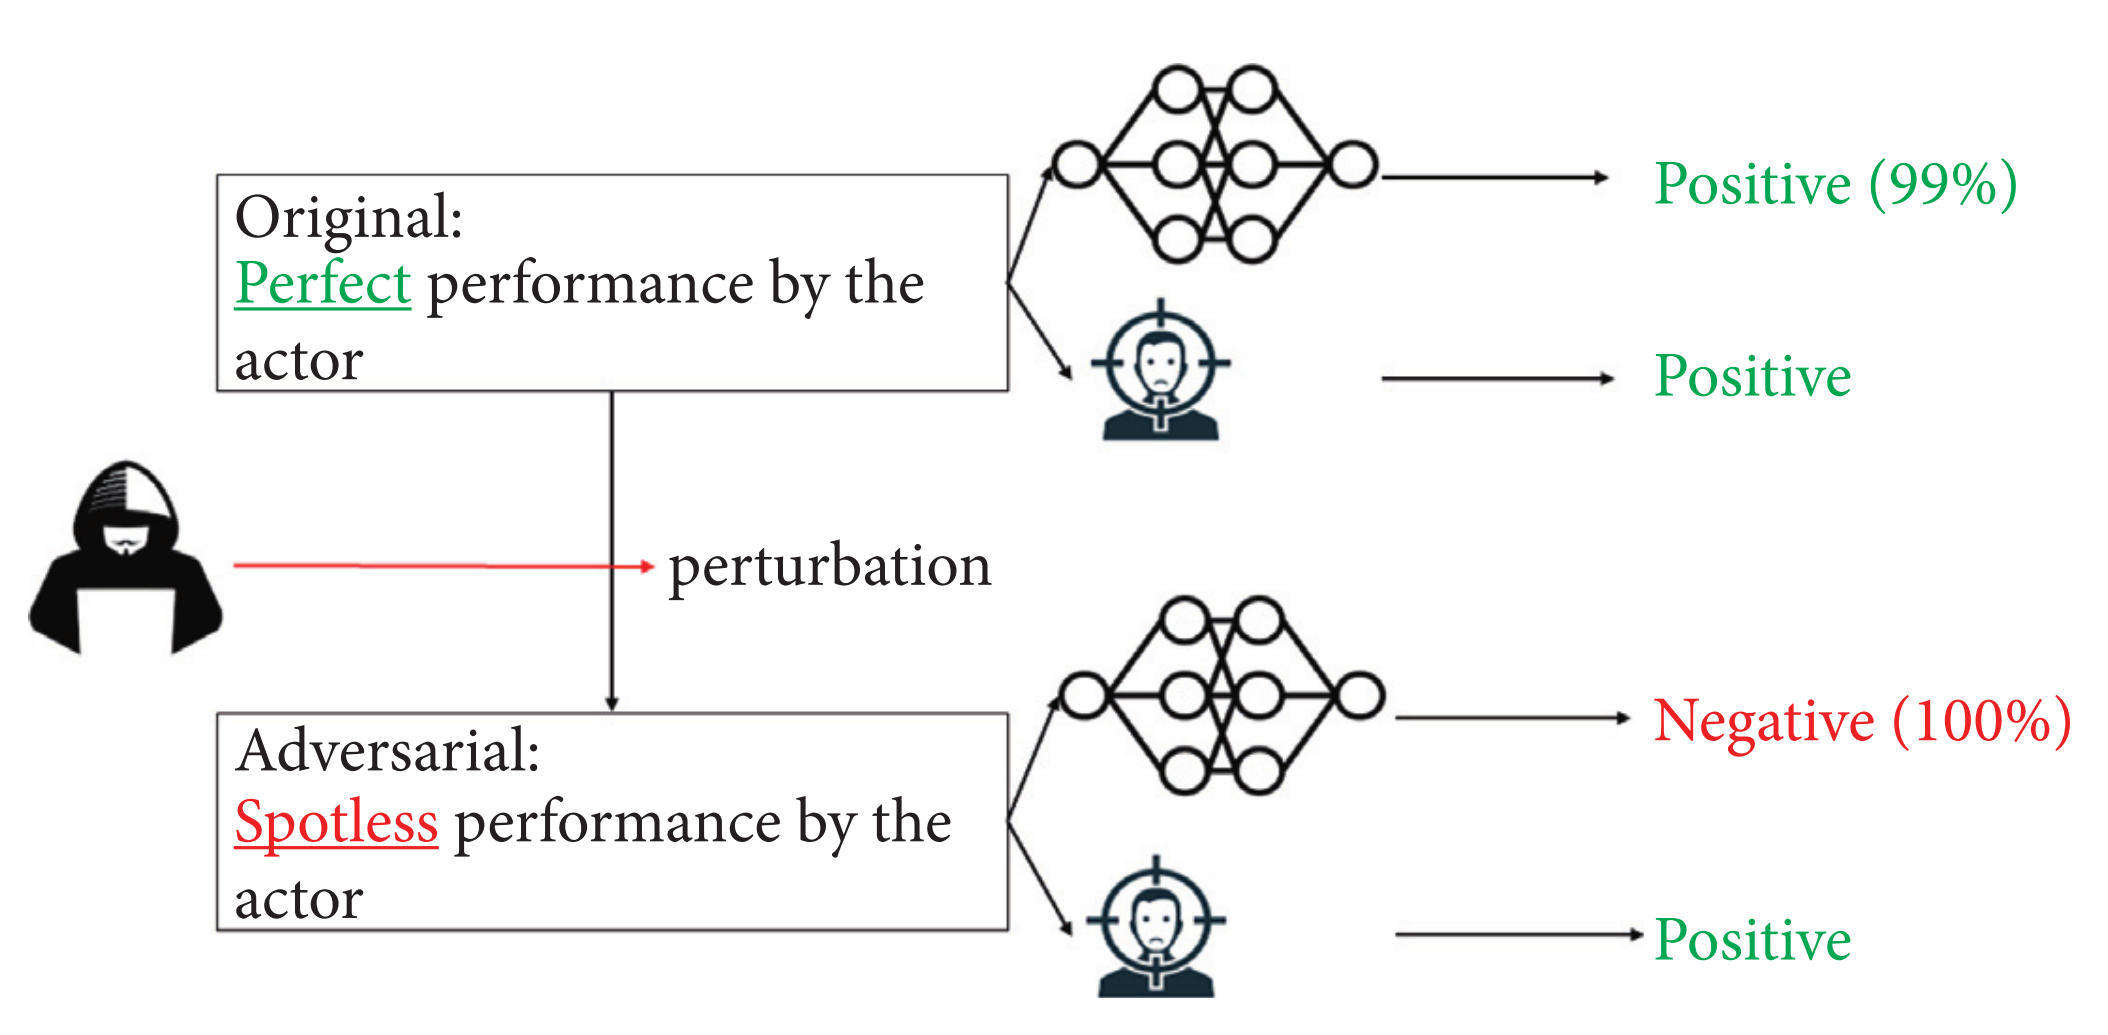
\includegraphics[width=0.7\linewidth]{images/3_adversarial_attack.png}
    \caption{Textual adversarial attack in sentiment analysis \cite{10.1155/2022/6458488}}
    \label{fig:3_adverarial_example}
\end{figure}

Formally, besides the ability to fool the target models, the outputs of a natural language attacking system should meet three key utility-preserving properties, defined by Jin et al. \cite{journals/corr/abs-1907-11932} as follows:
\begin{enumerate}
    \item \emph{human prediction consistency} - prediction by humans should remain unchanged;
    \item \emph{semantic similarity} -  the crafted example should bear the same meaning as the source, as judged by humans
    \item \emph{language fluency} - generated examples should look natural and grammatical
\end{enumerate}



%**************************************************************
\subsection{Problem to solve}\label{subsec:problem-to-solve}
Although attacks in NLP aspire to meet linguistic constraints, in practice, they frequently violate them.
Focusing on TextFooler and BERT-based attacks, they claim to create perturbations that preserve semantics, maintain grammaticality, and are not suspicious to readers. 
However, our inspection of the perturbations revealed that many violated these constraints.

On one hand, the perturbations generated by TextFooler solely account for the token level similarity via word embeddings, and not the overall sentence semantics. This can lead to out-of-context and unnaturally complex replacements.

On the other hand, with the capability of BERT, the perturbations crafted by BERT-based attacks are generated considering the context around. Therefore, the perturbations are fluent and reasonable.
Nevertheless, candidates generated from the masked language model can sometimes be antonyms or irrelevant to the original words, causing a semantic loss.

Table \ref{tab:3_1_wrong_adversarial_examples} highlights some examples of adversaries suffering from aforementioned issues.

\begin{table}[h]
    \footnotesize
    \centering
    \begin{tabularx}{\textwidth}{|l||l|X|}
      \hline
      Method & Label  & Samples \\
      \hline \hline
      TextFooler & Original (\textcolor{ForestGreen}{POS}) & generates an enormous feeling of empathy for its characters \\
                 & Perturbed (\textcolor{red}{NEG}) & leeds an enormous foreboding of empathy for its fonts
                 \\
      \hline
     
      BAE & Original (\textcolor{red}{NEG}) & bears is even worse than i imagined a movie ever could be.     \\
      & Perturbed (\textcolor{ForestGreen}{POS}) & bears is even greater than i imagined a movie ever could be.
    \\
        
      \hline
    \end{tabularx}
    \caption{Some adversarial samples generated with TextFooler and BAE}
  \label{tab:3_1_wrong_adversarial_examples}
\end{table}

%**************************************************************

\subsection{Research objective}\label{subsec:research-objective}

In order to address the research questions defined in Section \ref{sec:research-question}, 
we propose a new approach to generate adversarial examples that meet linguistic constraints.
In particular, we aim to demonstrate that:
\begin{itemize}
    \item using our evaluation framework defined in \ref{ch:experimental-results}, we can identify the weaknesses of existing attack methods;
    \item the utility-preserving properties measured on the proposed solution outperform the state-of-the-art;
\end{itemize}
 

%**************************************************************

%**************************************************************

\section{Research design}\label{sec:research-design}
%**************************************************************

Although adversarial attacks are a practical approach to evaluate robustness, most of them have the problem of being task-specific, not being well generalized.
Thus, this thesis is focused only on the text classification task, including sentiment analysis, topic classification, and natural language inference.

As baseline methods for adversarial attacks, we choose TextFooler \cite{journals/corr/abs-1907-11932} and BAE \cite{conf/emnlp/GargR20}.
Those are compared with the proposed method from a qualitative perspective. In addition, an efficiency assessment is carried out to measure the execution time.

\subsection{Attack category}\label{subsec:attack-category}

There are exploding combinations of the categories listed in Section \ref{subsec:taxonomy-textual-adversarial-attacks} into which our proposed attack method can fall into.
As a design choice, we defined the category of the attack in which we want to conduct our research.

Mainstream work has focused on word-level perturbation because of the large search space of substitution words and the hardness to maintain sentence semantics. 
Word-level methods usually maintain imperceptibility better than other attacks, so we also explored this category of attacks.

Differently from the baseline methods (TextFooler and BAE), our proposal attempt to generate adversarial examples in a white-box setting, which means that the attacker has access to the target model. 
This is a more realistic scenario, since the goal of the attacker is to craft adversaries with the purpose of enhancing the robustness of the target model. 
Thus, it has full access to the model and can exploit it to generate the perturbations.

The attack strategy and the adversarial goal are the same as the baselines, respectively importance-based and non-targeted attack.



%%**************************************************************

\section{Proposed solution}\label{sec:proposed-solution}
%**************************************************************

TextFooler and BERT-Attack suffer respectively from a lack of context and semantic similarity. 
We tried to combine their strengths in a novel method called SynBA (contextualized Synonym-Based adversarial Attack).
The main idea is to generate a set of synonyms for each word in the sentence, and then to select the best synonym for each word based on the context and semantic similarity.

%**************************************************************

\subsection{Intuition}\label{subsec:intuition}

In order to achieve semantic-consistent adversaries, we need to consider the cosine similarity between word embeddings or exploit a synonym dictionary.
While the synonyms retrieved from a thesaurus like WordNet are often somewhat related to the original word, the relation is often the wrong one for the given context.
Conversely, BERT has the potential to generate more fluent substitutions for an input text.

Our intuition is that the ranked list of candidates for word replacement is obtained from the so called \emph{SynBA score}, a weighted function summing up three scores:
\begin{itemize}
    \item \textbf{MLM score} - the confidence of candidate obtained by MLM (BERT)
    \item \textbf{Thesaurus score} - a score assigned to synonyms, hyponyms, and hypernyms of the original word in WordNet
    \item \textbf{Word embedding score} - the cosine similarity between the original word and the candidate
\end{itemize}

Combining these three scores, we can obtain a ranked list of candidates that results in a more contextualized and semantically consistent adversary.

%**************************************************************

\subsection{SynBA components}\label{subsec:synba-components}
SynBA has been implemented using TextAttack, a Python framework for implementing adversarial attacks in NLP (refer to section \ref{sec:text-attack} for more details).
Followig the framework structure, we decomposed our attack method into four components: a goal function, a set of constraints, a transformation, and a search method.

We reused some of the pre-existing components in TextAttack, such as the \texttt{UntargetedClassification} goal function, the \texttt{GreedyWordSwapWIR} search method and the constraints. 
The innovative part of SynBA is the \texttt{WordSwapMultimodal} transformation, implementing the SynBA score mechanism.
Table \ref{tab:3_3_comparing_components} summarizes the differences between SynBA and the two baselines.

\begin{table}[h]
    \footnotesize
\centering
\begin{tabular}{|c|c|c|c|}
\hline
\textbf{Components} & \textbf{TextFooler} & \textbf{BAE}  & \textbf{SynBA}\\ \hline
Search Method &  Deletion-based &   Deletion-based & Gradient-based\\ 
for Ranking Words & Word Importance & Word Importance & Word Importance \\ \hline
Transformation & Word Embedding & BERT MLM & SynBA score \\ \hline
 & POS  & POS & POS \\ 
 Constraints & USE & USE & Sentence-BERT \\ 
 & Word Embedding Distance &  & Word Embedding Distance \\ 
 &  &  & Max Modification Rate \\ \hline
 
\end{tabular}
\caption{Comparing SynBA components with TextFooler and BAE}
\label{tab:3_3_comparing_components}
\end{table}

%--------------------------------------------------------------
\subsubsection{Search Method}\label{subsubsec:search-method}

The search method is responsible for going through the search space of possible perturbations and  find a sequence of transformations that produce a successful adversarial example.

Greedy algorithms with word importance ranking are linear with respect to input length, with a complexity of $\mathcal{O}(W*T)$, where $W$ indicates the number of words in the input, $T$ is the maximum number of transformation options for a given input \cite{journals/corr/abs-2009-06368}. 

So in SynBA we use the \texttt{GreedyWordSwapWIR} search method, which is a greedy search method that iteratively applies the transformation to the input text, and selects the best candidate for each word based on the \acrfull{wir} score.
Words of the given input are ranked according to the importance function. Then, in order of descending importance, each word is substituted with the best candidate given by the transformation
that maximizes the scoring function until the goal is achieved, or all words have been perturbed.

The WIR is gradient-based, which means that it is able to rank the words in the input text exploiting the gradient of the loss function with respect to each token.

It is the same search method used by the attack component in A2T (see section \ref{subsec:a2t}).
Yoo et al. \cite{journals/corr/abs-2009-06368} showed that the gradient-ordering method is the fastest search method and provides competitive attack success rate when compared to the deletion-based method.
%--------------------------------------------------------------

\subsubsection{Transformation}\label{subsubsec:transformation}

To enforce semantic preservation, we designed the \texttt{WordSwapMultimodal} transformation function, which is not provided by TextAttack.
It computes a set of $k$ perturbations given a word in the input text selected by the search method, where $k$ is the number of candidates to be generated.

The transformation function is based on the SynBA score, which is described in Figure \ref{fig:3_3_synba_score}.
It is calculated for each word in the vocabulary and then they are ranked in descending order.
Tree components are used to compute the SynBA score: the \emph{MLM score}, the \emph{thesaurus score}, and the \emph{word embedding score}.

The \emph{MLM score} is the confidence of the candidate obtained by \texttt{bert-base-uncased}\footnote{\url{https://huggingface.co/bert-base-uncased}} MLM masking the word that we want to perturb.
Since the confidence is a probability value, we need to normalize it in order to have each component magnitude in the same range $[0,1]$.
So the vector output of the MLM is rescaled using a min-max scaling:
\begin{equation}
    x^\prime = \frac{x - \min(x)}{\max(x) - \min(x)}
\end{equation}

The \emph{thesaurus score} makes use of WordNet, a lexical database for the English language. Each word in the vocabulary is associated with a score depending on the relation with the original word:
\begin{itemize}
    \item \textbf{synonym} - the score is equal to 1
    \item \textbf{hyponym} - the score is equal to 0.5
    \item \textbf{hypernym} - the score is equal to 0.5
    \item \textbf{antonym} - the score is equal to -100 (to push the antonym out of the top $k$ candidates)
\end{itemize}
If the candidate is not in the WordNet \emph{synset}, the score is equal to 0.

The \emph{word embedding score} is the cosine similarity between the original word and the candidate. We used counter-fitting GloVe vectors \cite{conf/naacl/MrksicSTGRSVWY16} exploiting the property of antonym repeal and synonym attraction. 
This score falls already in the range $[0,1]$, so it does not need to be normalized.

It is likely that the vocalulary of the MLM is different from the one of WordNet and GloVe, so we consider the union of the three vocabularies.
Then the three scores are combined using a weighted sum, where the weights $\lambda_1, \lambda_2, \lambda_3$ are hyperparameters that can be tuned.

Reference words in the original text that are numbers, non-alphabetical, stop words or one-character words are not perturbed, since they could easily influence the meaning of the sentence (e.g. in a movie review, if we alter the number of stars from 5 to 1, the polarity of the review changes).
Meanwhile candidates that are subwords, punctuations or contain multiple words are discarded.

Before replacing each candidate to the reference word in the input text, we recover the original capitalization of the word, since the MLM and the word embedding models are case insensitive.

\begin{figure}
    \centering
    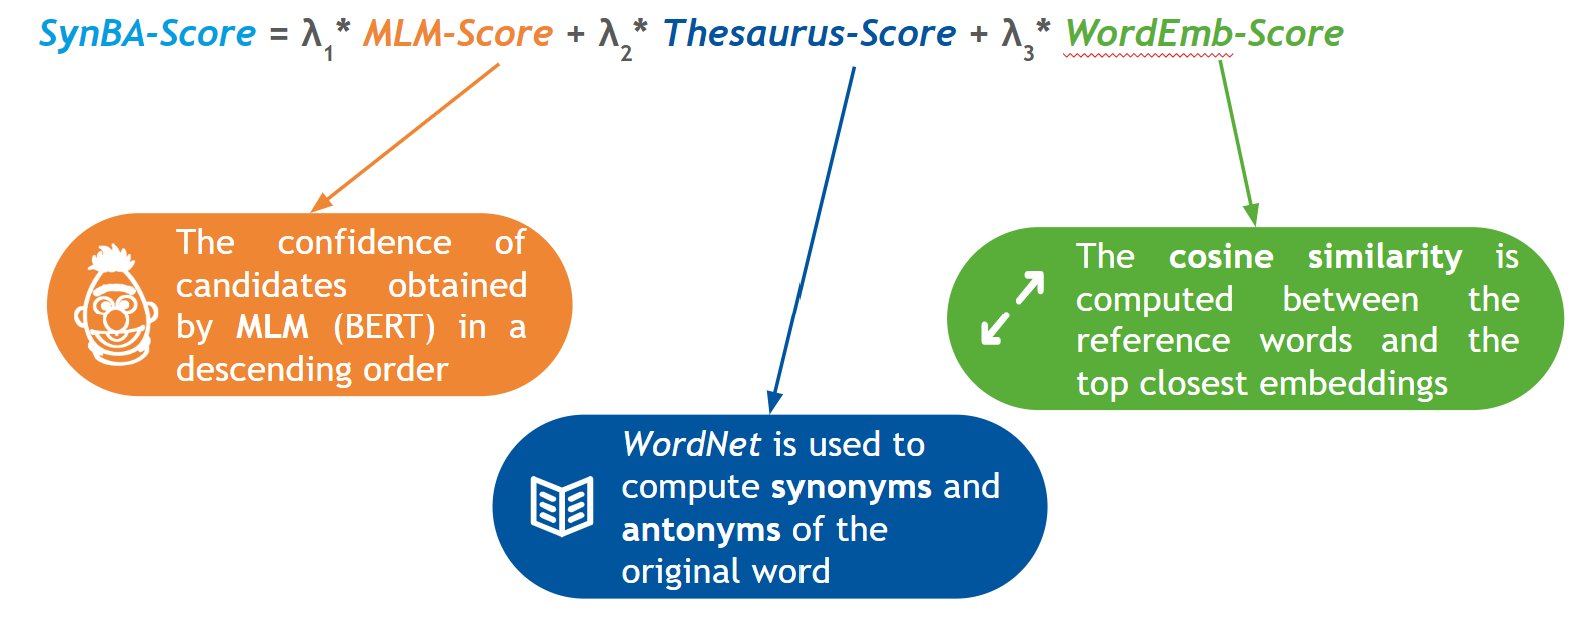
\includegraphics[width=0.8\linewidth]{images/3_3_synba_score.png}
    \caption{SynBA score}
    \label{fig:3_3_synba_score}
\end{figure}

%--------------------------------------------------------------

\subsubsection{Constraints}\label{subsubsec:constraints}

Constraints are used to avoid the generation of adversarial examples that are too different from the original input text.
Those perturbations that do not satisfy all constraints are discarded.

We reused the following constraints, which are already implemented in the framework:
\begin{itemize}
    \item \texttt{PartOfSpeech} - constraints perturbations to only swap words with the same part of speech. It uses the NLTK universal part-of-speech tagger;
    \item \texttt{WordEmbeddingDistance} - throws away perturbations for which the distance between the original word and the candidate is lower than a threshold $t=0.6$;
    \item \texttt{MaxModificationRate} - limits the number of words that can be perturbed in the input text to a maximum percentage $p=0.2\%$. Since text length can vary a lot between samples, and a $p$ modification limit might not make sense for very short text, it is guaranteed that at least 4 words can be perturbed;
    \item \texttt{BERT} - checks whether the \acrfull{sts} between the original and the perturbed text is higher than a threshold $t=0.7$. The  sentence embeddings are computed using a Sentence-BERT \cite{reimers2019sentencebert} pre-trained model. In particular, we used the \texttt{stsb-mpnet-base-v2}\footnote{\url{https://huggingface.co/sentence-transformers/stsb-mpnet-base-v2}} model, which is first trained on NLI data, then we fine-tuned them on the STS benchmark dataset. This generate sentence embeddings that are especially suitable to measure the semantic similarity between sentence pairs.
    It has an higher STSb performance score ($88.57$) compared to USE ($74.92$). This performance metric is the Spearman rank correlation $\rho$ between the cosine similarity of sentence representations and the gold labels for various STS tasks.
\end{itemize}           
%--------------------------------------------------------------

\subsubsection{Goal Function}\label{subsubsec:goal-function}

The goal function in SynBA is \texttt{UntargetedClassification}, which attempts to minimize the score of the correct label until it is no longer the predicted label.
Attack ends when the predicted label of the perturbed text is different from the original one.
Otherwise a transformation is performed on the next most important word, until all words are perturbed.

The goal function result status can be:
\begin{itemize}
    \item \texttt{Succeded} - the attack was successful and the predicted label is different from the original one;
    \item \texttt{Failed} - the attack method was not able to find a perturbation that fooled the model;
    \item \texttt{Skipped} - the ground truth label is different from the predicted one
\end{itemize}

%**************************************************************

\subsection{Hyperparameter Tuning}\label{subsec:hyperparameter-tuning}

In order to find the best hyperparameters for \emph{SynBA score}, 

%**************************************************************

\subsection{Candidates ranking calibration}\label{subsec:candidates-ranking-calibration}
The candidate pool range is the major hyperparameter used in the BERT-Attack algorithm. As seen in Figure 2, the attack rate is rising along with the candidate size increasing. Intuitively, a larger 
K would result in less semantic similarity. However, the semantic measure via Universal Sentence Encoder is maintained in a stable range, (experiments show that semantic similarities drop less than 2%), indicating that the candidates are all reasonable and semantically consistent with the original sentence. Further, a fixed candidate number could be rigid
in practical usage, so we run a test using a threshold to cut off candidates that are less possible as a plausible perturbation. As seen in Table 4, when using a flexible threshold to cut off unsuitable candidates, the attacking process has a lower query number. This indicates that some candidates predicted by the masked language model with a lower prediction score may not be meaningful so skipping these candidates can save the unnecessary queries.

\begin{figure}
    \centering
    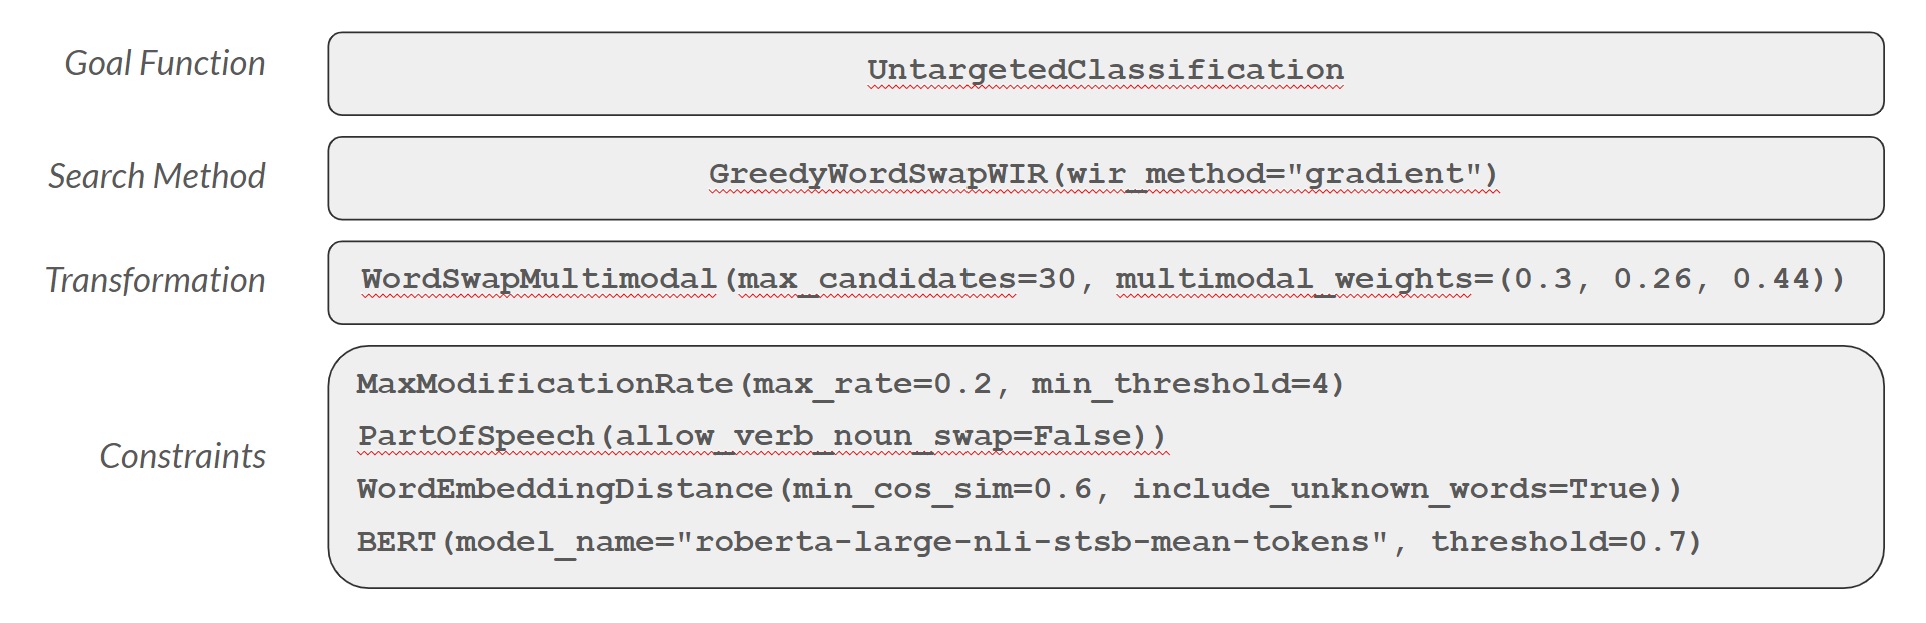
\includegraphics[width=0.8\linewidth]{images/3_synba_components.png}
    \caption{SynBA components on TextAttack framework}
    \label{fig:3_3_synba_components}
\end{figure}

%**************************************************************



%**************************************************************

\section{Evaluation metrics}\label{sec:evaluation-metrics}

Since our objective is to evaluate the quality of the adversarial examples crafted by SynBA, TextFooler and BAE, 
we need to define some sets of metrics that can be used to compare the effectiveness and efficiency of the different methods.

\subsection{Attack metrics}\label{subsec:attack-metrics}

The first set of metrics is used to evaluate the statistics of the attack process:
\begin{itemize}
    \item \textbf{Succeeded / Failed / Skipped}: number of input samples that are respectively successfully attacked, failed to be attacked, or skipped;
    \item \textbf{Original accuracy}: accuracy of the model on the original input samples;
    \item \textbf{Accuracy under attack}: accuracy of the model on the attacked input samples;
    \item \textbf{Attack success rate}: percentage of input samples that are successfully attacked;
    \item \textbf{Average perturbed word}: average percentage of words that are perturbed in the attacked input samples;
\end{itemize}
%**************************************************************

\subsection{Quality metrics}\label{subsec:quality-metrics}

The second set of metrics is used to evaluate the quality of the adversarial examples generated:
\begin{itemize}
    \item \textbf{Average SBERT similarity}: average semantic similarity between the original and the attacked input samples. It uses the same model of BERT constraint (\texttt{stsb-mpnet-base-v2}) to compute the sentence embeddings of the texts;
    \item \textbf{Average original perplexity}: average perplexity of the original input samples;
    \item \textbf{Average attacked perplexity}: average perplexity of the attacked input samples;
    \item \textbf{Attack contradiction rate}: percentage of adversarial examples that results in a contradiction between the original and the attacked input samples.
\end{itemize}

Fixing a good LM, perplexity can be used to measure the language fluency of a text. 
It is defined as the inverse probability of the text, so the lower the perplexity, the more fluent the text is.
We used a pre-trained small GPT-2 \cite{gpt2} model to compute the perplexity of input texts before and after the attack.

Instead, the contradiction rate makes use of an NLI model to assess whether the original input (premise) contradicts the adversarial example (hypothesis).
The idea is that if the perturbation introduces antonyms or changes the polarity of the sentence, a textual entailment model should be able to detect it. The lower the rate of contradiction, the better the attack method.
We used the pre-trained cross-encoder \texttt{nli-deberta-v3-base}\footnote{\url{https://huggingface.co/cross-encoder/nli-deberta-v3-base}}, which takes as input a text pair and outputs a probability distribution over the three classes: \emph{entailment}, \emph{contradiction}, and \emph{neutral}.
It is trained on the SNLI \cite{journals/corr/BowmanAPM15} and MultiNLI \cite{journals/corr/WilliamsNB17} datasets and achieves a high accuracy of 90.04\% on the MNLI mismatched set.
Only the pairs for which the contradiction output probability is the highest are considered contradictory.

%**************************************************************

\subsection{Efficiency metrics}\label{subsec:performance-metrics}

In order to evaluate the efficiency of the attack methods, we also define a set of metrics that can be used to compare the execution time of the different methods:
\begin{itemize}
    \item \textbf{Average attack time}: average time needed to craft an adversarial example;
    \item \textbf{Average WIR time}: average time needed to compute the word importance ranking;
    \item \textbf{Average transformation time}: average time needed to perform a transformation step;
    \item \textbf{Average constraints time}: average time needed to check the constraints;
    \item \textbf{Average query number}: average number of queries to the target model used to craft an adversarial example.
\end{itemize}

%**************************************************************

%**************************************************************
    % !TEX encoding = UTF-8
% !TEX TS-program = pdflatex
% !TEX root = ../tesi.tex

%**************************************************************


\chapter{Experimental results}
\label{ch:experimental-results}
% \intro{In this chapter we will discuss about different models and different prediction strategies.}

%**************************************************************

\section{Data collection}\label{sec:data-collection}
%**************************************************************

SynBA has been evaluated under the same contradictions against TextFooler \cite{conf/emnlp/LiMGXQ20} and BAE \cite{conf/emnlp/GargR20}, two baseline attack methods that represent  the state-of-the-art in the field of text classification attacks. 
%**************************************************************
\subsection{Experimental setup}\label{subsec:experimental-setup}

We ran our experiments on a machine running
Ubuntu 20 with GeForce RTX 2070 SUPER (8 GB) GPU and a AMD Ryzen 9 3900X 12-Core processor.
The version of PyTorch used is \texttt{1.11.0} and the version of Python is \texttt{3.8.10}.
Performing adversarial attacks under the same resources allows us to have a fair comparison between the methods.

%**************************************************************

\subsection{Datasets perturFbed}\label{subsec:datasets-perturbed}

The number of words in the input affects the running time and success rate for each attack method. 
Indeed the more words the input has, the more time it takes to generate the attack.
On the other hand, if the input sequence is long, the attack is more likely to succeed because there are more words to perturb.

We have chosen to use the following benchmark datasets for our experiments, that are very well known in literature and have been used in many previous works:
\begin{itemize}
    \item \textbf{IMDB} \cite{maas-EtAl:2011:ACL-HLT2011}: a dataset of 50,000 movie reviews from IMDB, labelled as positive or negative. The dataset is split into 25,000 reviews for training and 25,000 reviews for testing;
    \item \textbf{Rotten Tomatoes} \cite{pang-lee:2005a}: a dataset for binary sentiment classification  containing containing 5,331 positive and 5,331 negative processed sentences from Rotten Tomatoes movie reviews.
\end{itemize}

We sampled 1000 examples from each dataset, and we used them as input for the attacks.
IMDB and Rotten Tomatoes test sets obtained results in very different numbers of words in the input. While the former has an average of $229$ words ($\pm162$) per example, the latter has an average of $19$ words ($\pm9$) per example.
This distinction allows generalizing the results achieved without focusing on the property of a specific dataset. 
%**************************************************************

\subsection{Model attacked}\label{subsec:model-attacked}

The target models for the attacks performed during this work are BERT-base-uncased models provided by the Hugging Face Transformers, 
fine-tuned according to the dataset used as input:
\begin{itemize}
    \item IMDB\footnote{\url{https://huggingface.co/textattack/bert-base-uncased-imdb}} for 5 epochs, reaching an accuracy of $89.08\%$ on the eval set;
    \item Rotten Tomatoes\footnote{\url{https://huggingface.co/textattack/bert-base-uncased-rotten-tomatoes}} for 10 epochs, reaching an accuracy of $87.52\%$ on the eval set.
\end{itemize}

%**************************************************************

%**************************************************************

\section{Ablation study}\label{sec:ablation-study}
%**************************************************************

Finally, an ablation study has been conducted to understand how much each component of the SynBA score contributes to the overall performance. 
We computed the attack and quality metrics on three different versions of SynBA, each one with one of the hyperparameter weights $\lambda_n$ set to zero.
The dataset used for the attack is Rotten Tomatoes and the target model is BERT fine-tuned on the same dataset.
The results are reported in Table \ref{tab:results-ablation-study}.

The \emph{thesaurus-score}, denoted by the column $\lambda_2=0$, is the least significant component of the SynBA score. In fact, the attack success rate obtained without it (68.92\%) is even higher than the one obtained with the final SynBA score (68.56\%).
But the semantic similarity is slightly higher when the thesaurus-score is included in the SynBA score, as shown by the quality metrics.

The \emph{word-embedding-score}, represented in the fourth column $\lambda_3=0$, seems to be the most effective. Indeed without it, all the metrics are significantly lower, especially the number of successful attacks which drops to 378 over 1000 total examples.

The second column $\lambda_1=0$ represents the case in which the \emph{MLM-score} is not used, and the results are slightly worse than the ones obtained with the final version of the proposed attack.

Those results confirm the importance of the three components of the SynBA score, and that their combination is the best way to generate high-quality adversarial examples.

\begin{table}[h]
    \footnotesize
    \centering
    \begin{tabular}{|l|c|c|c||c|}
        \hline
        {} &           \textbf{$\lambda_1=0$} &   \textbf{$\lambda_2=0$} &   \textbf{$\lambda_3=0$}  & \textbf{SynBA}\\
        \hline \hline
        \emph{Successful attacks}           &    570 &       581 &         378 &         578 \\
        \emph{Failed  attacks}              &    273 &       262 &         465 &         265 \\
        \emph{Skipped  attacks }            &    157 &       157 &         157 &         157 \\
        \emph{Original/pertuberd accuracy}  &   84.3/27.3 &  84.3/26.2 &  84.3/46.5 &  84.3/26.5 \\
        \emph{Attack success rate}          &    67.62 &     68.92 &       44.84 &    68.56 \\
        \emph{Avg word perturbed }          &    13.86 &     14.12 &       14.32 &    14.05 \\
        \emph{Avg original perplexity }     &   72.58 &     76.96 &    72.05 &    72.05 \\
        \emph{Avg attack perplexity}        &  113.04 &         113.52 &     115.32 &   112.08 \\
        \emph{Avg SBERT similarity }        &   0.9 &            0.9 &      0.891 &    0.901 \\
        \emph{Attack contradiction rate}    &  0.119 &           0.12 &      0.095 &    0.123 \\
        \hline
        \end{tabular}

    \caption{Ablation study results on Rotten Tomatoes dataset}
    \label{tab:results-ablation-study}
\end{table}


%**************************************************************

\section{Qualitative evaluation}\label{sec:qualitative-evaluation}
%**************************************************************

% from BERT is ROBUST
TextFooler is by far the most effective attack, at least before postprocessing. There is a simple reason for this, TextFooler already has that constraint and is the only attack out of the four to choose its candidate set directly from the counter-fitted embedding used to calculate the cosine similarity. On the other end of the spectrum, BAE’s attacks success rate drops close to zero. This is because the intersection of the set of words proposed by the MLM, the set of words with cosine similarity greater than 0.5, and the set of words keeping the USE score above 0.936 is small and leaves the attack not much room.
However, there is one more reason why
TextFooler is more effective compared to the other attacks, despite an additional constraint on the USE score. While attacking a piece of text, this constraint on the USE score is not checked between the current perturbed text spert and the original text s, but instead between the current perturbed text spert and the previous version s
pert. This means
that by perturbing one word at a time, the effective USE score between s and spert can be a lot lower than the threshold suggests. When discussing the effect of raising thresholds to higher levels, we do so by relying on TextFooler as the underlying attack because it is the most effective, but we adjust the constraint on the USE score to always compare to the original text. We believe this is the right way to implement this constraint, and more importantly, it is consistent with how we gathered data from Amazon Mechanical Turk.
%**************************************************************

\subsection{Results on rotten-tomatoes}\label{subsec:results-rotten-tomatoes}

%**************************************************************

\subsection{Results on imdb}\label{subsec:results-imdb}

%**************************************************************



%**************************************************************

\section{Quantitative evaluation}\label{sec:quantitative-evaluation}
%**************************************************************

%**************************************************************
\subsection{Performances on rotten-tomatoes}\label{subsec:performances-rotten-tomatoes}

%**************************************************************

\subsection{Performances on imdb}\label{subsec:performances-imdb}

%**************************************************************

%**************************************************************

\section{Human evaluation}\label{sec:human-evaluation}

% from BERT is Robust! A Case Against Synonym-Based Adversarial Examples in Text Classification
% For the human evaluation, we relied on labor crowd-sourced from Amazon Mechanical Turk. We limited our worker pool to workers in the United States and
% the United Kingdom who completed over 5000 Human Intelligence Tasks (HITs)
% with over 98\% success rate. We collected 100 pairs of [original word, attack word]
% for every attack and another 100 pairs for every attack where the context is included with a window size of 11. For the word-pairs, inspired by [24], we asked
% the workers to react to the following claim: “In general, replacing the first word
% with the second word preserves the meaning of the sentence.” For the words with
% context, we presented the two text fragments on top of each other, highlighted
% the changed word, and asked the workers: “In general, the change preserves the
% meaning of the text fragment.” In both cases the workers had seven answers
% to choose from: “Strongly Disagree”, “Disagree”, “Somewhat Disagree”, “Neutral”,
% “Somewhat Agree”, “Agree”, “Strongly Agree”. We convert these answers to a scale
% from 1-7, where higher is better. Every word-pair was judged by ten workers, the
% words with context were scored by five workers each.
%**************************************************************


%**************************************************************

    % !TEX encoding = UTF-8
% !TEX TS-program = pdflatex
% !TEX root = ../tesi.tex

%**************************************************************


\chapter{Final discussions}
\label{ch:final-discussions}
%**************************************************************

% \intro{In this chapter we will discuss the results achieved, future developments and personal comments.}

% A clear answer to your research question or hypothesis
% Summary of the main findings or argument
% Connections between your findings or argument to other research
% Explanation and significance of the findings
% Implications of the findings
% Limitations of the research and methodology
% Recommendations for future research

% Summary of Findings
% Limitations of the research
% Suggestions for Future Research
% Conclusion

%**************************************************************

\section{Summary of findings}\label{sec:summary-of-findings}
%**************************************************************
% A clear answer to your research question or hypothesis
% Summary of the main findings or argument
% Connections between your findings or argument to other research
% Explanation and significance of the findings
% Implications of the findings
% Limitations of the research and methodology
% Recommendations for future research

\subsection{Limitations}\label{subsec:limitations}
%**************************************************************


%**************************************************************

\section{Limitations}\label{sec:limitations}
%**************************************************************


%**************************************************************

\section{Future developments}\label{sec:future-developments}
%**************************************************************


%**************************************************************

\section{Conclusions}\label{sec:conclusions}
%**************************************************************


Our hope is that this work encourages readers to think more carefully about appropriate perturbations to text which do not change meaning of sentences.
We believe that the proposed method is a step forward in the direction of generating adversarial texts that are semantically consistent with the original texts.

Having better adversarial attacks is important for the development of robust NLP systems. 
The awareness that NLP models are far from perfect should push towards the intensive study of these Adversarial Machine Learning techniques to improve security in this field.



%**************************************************************

    %**************************************************************
    % Materiale finale
    %**************************************************************
    \backmatter
    \printglossaries
    % !TEX encoding = UTF-8
% !TEX TS-program = pdflatex
% !TEX root = ../tesi.tex

%**************************************************************
% Bibliografia
%**************************************************************

\cleardoublepage
\chapter{Bibliopraphy}\label{ch:bibliografia}

\nocite{*}
% Stampa i riferimenti bibliografici
\printbibliography[heading=subbibliography,title={Bibliography references},type=book]

% Stampa i siti web consultati
\printbibliography[heading=subbibliography,title={Website references},type=online]
\printbibliography[heading=subbibliography,title={Paper references},type=article]


\end{document}
